\chapter{Vapour-Liquid Equilibrium of Mixtures}\label{Section:04}

Up to this point, we have only considered thermodynamic and volumetric properties of pure components at prescribed pressure and temperature conditions. However, most engineering applications deals with mixtures of components that may be present in single or multiple phases, \eg oil in reservoirs, naphtha distillation, steel processing etc. This module focuses on understanding PVT behaviour of mixtures and the conditions for vapour-liquid equilibrium (VLE).


   
   
%%%
%%% SECTION
%%%
   \section{Gibbs Phase Rule}\label{Chapter:Introduction:Section:Gibbs_PhaseRule}\index{Gibbs phase rule}\index{Phase rule|see {Gibbs phase rule}}


%%%



%%% SECTION
\section{A Few Important Definitions}


%%% SUBSECTION
\subsection{Representing Compositions}\label{Section:04:Compositions}
In the previous modules, we mostly focused on thermodynamic properties of systems containing pure chemical species. This module (and the remaining of the course) will study systems with arbitrary number of components, and the quantification of each component at each phase. For a mixture containing $\mathcal{C}$ chemical species, each of them with an arbitrary number of moles, $n_{i},\;\;\forall i\in\left\{1,2,\cdots,\mathcal{C}\right\}$, 
\begin{subequations}
   \begin{enumerate}[a)]
       \item Molar (or mole) $\left(x_{i}\right)$ fraction:
            \begin{eqnarray}
                x_{i} = \frc{n_{i}}{n}.
            \end{eqnarray} 
            where $n=\summation[n_{i}]{i=1}{\mathcal{C}}$ is the total number of moles in the system. As the molar fraction is normalised, we can define:
            \begin{equation}
                  \summation[x_{i}]{i=1}{\mathcal{C}} = 1,
            \end{equation}
       \item (Average) Molar mass of mixtures:
            \begin{equation}
                \overline{MW} = \summation[\left(x_{i} \cdot MW_{i}\right)]{i=1}{\mathcal{C}}
            \end{equation}
         where $MW_{i}$ is the molecular weight (or molar mass) of species $i$.
   \end{enumerate}
\end{subequations}

%%% SUBSECTION
\subsection{Partial Molar Properties}\label{Section:04:PartialMolarProperties}

{\it Partial molar properties} describes the behaviour of homogeneous multi-component systems. Let's consider a homogeneous (\ie single phase) and open system (\ie system that allows mass and energy transfer across the boundary towards the surroundings) that undertakes a change in composition. Thus, the total value of any extensive property $M^{\text{t}}\;\left(M\equiv V, U, H, S, G, A\right)$ is not only a function of pressure and temperature, but it also depends on the number of moles of each species in the system. therefore
  \begin{subequations}
     \begin{equation}
        M^{\text{t}} = nM = M\left(T,P,n_{1},n_{2},\cdots, n_{\mathcal{C}}\right).\label{Mod04_PartialProperties1}
     \end{equation}
     The total derivative of Eqn.~\ref{Mod04_PartialProperties1} is,
     \begin{displaymath}  
        d(nM) = \Partial[(nM)]{P}{T,n}dP + \Partial[(nM)]{T}{P,n}dT + \Partial[(nM)]{n_{i}}{T,P,n_{j\ne i}}dn_{i},
     \end{displaymath}
     where the subscript $n$ in the partial derivatives indicates that the number of moles is kept constant, whereas $n_{j\ne i}$ indicates that the number of moles of all components, except component $i$, are kept constant. This expression can be simplified to be a function of the mole fraction, $x_{i}$,
     \begin{shaded}
        \begin{equation}  
           d(nM) = n\Partial[M]{P}{T,x}dP + n\Partial[M]{T}{P,x}dT + \summation[\overline{M}_{i}dn_{i}]{i}{},\label{Mod04_PartialProperties2}
        \end{equation}
     \end{shaded}
     \noindent where $\overline{M}_{i} = \Partial[(nM)]{n_{i}}{T,P,n_{j\ne i}}$ defines the {\it partial molar property} $\overline{M}_{i}$ of species $i$ in solution, \ie the change of the total property $nM$ of a mixture of $\mathcal{C}$ species resulting from the addition at constant $T$ and $P$ of infinitesimal amount of species $i$ to a prescribed amount of solution. We will discuss partial molar properties in more details in Module~\ref{Section:05}.
  \end{subequations}

%%% SUBSECTION
\subsection{Excess Properties}\label{Section:04:ExcessProperties}
  
In Section~\ref{Section:03:ResidualProperties}, we have defined {\it residual properties} for gases as the difference between any extensive thermodynamic property, $M$, in real gases and its equivalent assuming ideal gas behaviour, $M^{\text{ig}}$. The equivalent for liquids is called {\it excess properties}, \ie the deviation from an ideal liquid solution property.

Let's assume that $M$ is any extensive thermodynamic property (\eg $V$, $U$, $H$, $S$, $G$ and $A$), the excess property $M^{\text{E}}$ is defined as the difference between the property value of a solution and the value it would have as an ideal solution at the same $T$, $P$ and composition,
\begin{subequations}
  \begin{shaded}
    \begin{equation}
       M^{\text{E}} \equiv M - M^{\text{id}},\label{Mod04_ExcessProperties1a}
    \end{equation}
  \end{shaded}
  \noindent where properties in ideal ({\it id}) solutions of multiple chemical species can be represented as,
    \begin{displaymath}
       M^{\text{id}} = \summation[x_{i}M_{i}]{i}{},
    \end{displaymath}
    where $M_{i}$ is an extensive {\it molar property of the \underline{pure} chemical species}. For example, if we mix equal volumes of two species (\eg water and ethanol), the final volume \underline{is not} the sum of the individual volumes. In fact, the final volume will be slightly larger than the sum of the individual volumes and this is due to the non-ideality behaviour of real liquid fluids. Thus for a binary solution,
    \begin{equation}
      V^{\text{E}} = V - V^{\text{id}} = V - \summation[x_{i}V_{i}]{i}{} = V -\left(x_{1}V_{1}+x_{2}V_{2}\right).\label{Mod04_ExcessProperties1b} 
    \end{equation}
    %This equation shows that the total volume of a mixture of two components is different from the simple addition of both individual volumes. 
\end{subequations}



%%% SECTION
\section{Criteria for Chemical Equilibrium}\label{Section:04:ChemicalEquilibrium}

  
%%% SUBSECTION
\subsection{Chemical Potential $\left(\mu_{i}\right)$}\label{Section:04:ChemicalPotential}

If we apply the concept of partial molar property to the Gibbs free energy definition, assuming that this thermodynamic potential is a function of $P$, $T$ and $n$, \ie $G^{\text{t}}= nG = G\left(T,P,n_{1},n_{2},\cdots,n_{\mathcal{C}}\right)$,
  \begin{subequations}
      \begin{equation}
         d(nG) = n\Partial[G]{P}{T,x}dP + n\Partial[G]{T}{P,x}dT + \summation[\overline{G}_{i}dn_{i}]{i}{}.\label{Mod04_ChemPotentialDef1}
      \end{equation}
      By definition the {\it partial molar Gibbs free energy} is called \blue{chemical potential $\left(\mu_{i}\right)$},
      \begin{shaded}
         \begin{equation}
            \mu_{i} = \Partial[(nG)]{n_{i}}{T,P,n_{j\ne i}} \;\;\Longleftrightarrow\;\; \mu_{i} = \overline{G}_{i}.\label{Mod04_ChemPotentialDef1b}
         \end{equation}
      \end{shaded}
      The chemical potential can be understood as an energy associated with interactions of atoms/molecules in a mixture that controls the tendency of molecules to leave the solution (or return to the solution), and to chemically react. We have defined the Gibbs free energy in Eqn.~\ref{Mod03_GibbsFundamentalRelation01} as a function of $T$ and $P$, now we will extend it to be also a function of the number of moles of chemical species -- Eqn.~\ref{Mod04_ChemPotentialDef1},
      \begin{equation}
         d(nG) = (nV)dP - (nS)dT + \summation[\mu_{i}dn_{i}]{i}{},\label{Mod04_ChemPotentialDef1c}
      \end{equation}
      considering $n=1\;\Rightarrow n_{i}=x_{i}$, and Eqn.~\ref{Mod04_ChemPotentialDef1c} becomes
      \begin{shaded}
        \begin{equation}
          \blue{dG = VdP -SdT + \summation[\mu_{i}dx_{i}]{i}{}},\label{Mod04_ChemPotentialDef1d}
        \end{equation}
      \end{shaded}
  \end{subequations}
  
%%% SUBSECTION
\subsection{Thermodynamic Equilibrium}\label{Section:04:thermodynamicEquilibrium}

There are two main conditions for a system to achieve {\it chemical equilibrium}:
  \begin{enumerate}[a)]
     \item all distinct $\mathcal{P}$ phases that may co-exist are in equilibrium with each other, as such as there is no net mass transfer of any chemical species between phases;
     \item all chemical reactions that may occur between species are also in equilibrium, \ie there is no net progress \wrt conversion of reactants to products (and {\it vice-versa}).
  \end{enumerate}

  \begin{subequations}

    \medskip

    Let's initially consider a closed system (either homogeneous or heterogeneous) in thermal and mechanical equilibrium with the surroundings. In addition, let's also assume that the system is not under chemical equilibrium, \ie there are effective mass transfer across the phase boundary. Such transfer of matter occurs `till the point when the system is also at chemical equilibrium. In reality, these changes towards chemical equilibrium occur by infinitesimal gradients and are, therefore, irreversible. Applying the {\it First Law},
    \begin{displaymath}
      dU^{\text{t}} = dQ + dW\;\;\;\text{ with }\;\;\; dW = -PdV^{\text{t}},
    \end{displaymath}
    with the heat exchange between the system and the surroundings,
    \begin{displaymath}
      dS_{\text{surr}} = \frc{dQ_{\text{surr}}}{T_{\text{surr}}} = - \frc{dQ^{\text{t}}}{T},\;\;\text{ where } dQ_{\text{surr}} = - dQ^{\text{t}}.
    \end{displaymath}
    However, by the Second Law, $dS_{\text{surr}}+dS^{\text{t}} \ge 0$, and if we combine the expressions above $ - \frc{dQ^{\text{t}}}{T}+dS^{\text{t}}\ge 0$,
    \begin{displaymath}
      dQ^{\text{t}} \leq TdS^{\text{t}},
    \end{displaymath}
    \ie for every allowed change in state, the system can not spontaneously leave the current state. The system is said to be at \underline{stable equilibrium}.
    \begin{shaded}
      The \underline{entropy} of an adiabatically (\ie $dS<0$) isolated stable equilibrium system is \underline{maximum}.
    \end{shaded}
    We can write the criterion for stable equilibrium in non-adiabatic system from the First Law for $n$ moles,
    \begin{eqnarray}
      dQ = dU + PdV -\mu dn &\leq& TdS \label{Mod04_EquilibriumCriteria0} \\
      dU + PdV -\mu dn - TdS &\leq& 0,\label{Mod04_EquilibriumCriteria1}
    \end{eqnarray}
    thus,
    \begin{enumerate}[i)]
        \item if we make $U$, $V$ and $n$ constants, $dQ=0$ and the stability condition becomes \underline{$dS \ge 0$} $\Longrightarrow$ \underline{$S$ is maximum};
        \item if $S$, $V$ and $n$ are set as constants, then from Eqn.~\ref{Mod04_EquilibriumCriteria1}, the system will be stable if \underline{$dU\le 0$} $\Longrightarrow$ \underline{$U$ is minimum};
        \item if $T$, $V$ and $n$ are kept constants, then Eqn.~\ref{Mod04_EquilibriumCriteria1}, becomes
            \begin{eqnarray}
              dU - TdS &\leq& 0 \nonumber \\
              d(U-TS) &\leq& 0 \;\;  \text{(for } T \text{  constant}),
            \end{eqnarray}
            however, we have seen the definition of the Helmholtz free energy, $U-TS =A$, thus $dA\leq0$ $\Longrightarrow$ \underline{$A$ is minimum};
        \item from the Helmholtz free energy definition,
            \begin{eqnarray}
              dA &=& \overbrace{dU}^{\text{from Eqn.~\ref{Mod04_EquilibriumCriteria0}}: dU = dQ -dW +\mu dn} -SdT - TdS \nonumber \\
                &=& \red{dQ} -dW + \mu dn -SdT \red{-TdS},\label{Mod04_EquilibriumCriteria2}
            \end{eqnarray}
            from the Clausius inequality, $dQ-TdS \leq 0$, and if we consider $T$ and $n$ constants $\Longrightarrow\;\; dA = -dW + (dQ - TdS) \leq 0$, therefore
            \begin{displaymath}
                 dA \leq -dW \;\;\;\text{ or }\;\;\; W \leq -\Delta A.
            \end{displaymath}
            This means that $-\Delta A$ is the maximum work we can obtain from a process performed under constant $T$ and $n$ conditions. Also, as $A$ is a \underline{state function}, it does \underline{not} depend on the path, but only on the initial and final states;
         \item assuming $S$, $P$ and $n$ are kept constant, then Eqn.~\ref{Mod04_EquilibriumCriteria1} becomes
            \begin{displaymath}
                 d(U+PV) = dH \leq 0,
            \end{displaymath}
            for stable equilibrium $\Longrightarrow$ \underline{enthalpy is minimum};
         \item now, suppose that $T$, $P$ and $n$ are held constant, Eqn.~\ref{Mod04_EquilibriumCriteria1} becomes,
            \begin{displaymath}
                 d(U+PV-TS)  \leq 0,
            \end{displaymath}
            but $U+PV-TS = H-TS = G$, \ie \underline{the Gibbs free energy is minimum} for stable equilibrium with fixed $T$, $P$ and $n$.    
    \end{enumerate}
    In Table~\ref{Mod04_TableEquilibriumCriteria}, the \blue{equilibrium criteria} is summarised for all thermodynamic potentials. The stability criteria for \blue{Gibbs free energy} is particularly important for several chemical engineering processes involving closed systems, as so as we can state,

    \begin{shaded}
         `The equilibrium state of a closed system is that state for which the total Gibbs free energy is a minimum \wrt all possible changes at the given $T$ and $P$.'
      \end{shaded}
    
    \begin{table}
    \begin{center}
      \begin{tabular}{c c c c c}
         \hline
          Held            & State    &  Definition & Differential         &  Stable Equilibrium \\
          Fixed           & Function &             &                      &   Criterion          \\
          \hline
          $U$, $V$, $n$   & $S$      & --          & $dS=\frac{dQ}{T}$    & Maximum             \\
          $S$, $V$, $n$   & $U$      & --          & $dU=TdS-PdV+\mu dn$ & Minimum             \\
          $S$, $P$, $n$   & $H$      & $H\equiv U+PV$& $dH=TdS+VdP+\mu dn$ & Minimum             \\
          $T$, $V$, $n$   & $A$      & $A\equiv U-TS$& $dA=-SdT-PdV+\mu dn$ & Minimum             \\
          $T$, $P$, $n$   & $G$      & $G\equiv H-TS$& $dG=-SdT+VdP+\mu dn$ & Minimum             \\
      \end{tabular}
    \end{center}
    \caption{Criteria for thermodynamic equilibria.}\label{Mod04_TableEquilibriumCriteria}
    \end{table}
    
  \end{subequations}

%%% SUBSECTION
\subsection{Chemical Potential and Thermodynamic Equilibrium}\label{Section:04:ChemPotThermEquil}

Now, let's consider a closed system consisting of two phases in equilibrium  (vapour and liquid, or solid and vapour or liquid and solid), $\alpha$ and $\beta$. Each of these phases may be considered as an open system with an interface between them, where mass and energy can flow freely. Also, both systems (or phases) are in mechanical and thermal equilibrium $\left(\ie\; T^{\alpha}=T^{\beta}=T\text{ and } P^{\alpha}=P^{\beta}=P\right)$. We can apply Eqn.~\ref{Mod04_ChemPotentialDef1c} to both phases,
  \begin{subequations}

     \begin{eqnarray}
        d(nG)^{\alpha} &=& (nV)^{\alpha}dP - (nS)^{\alpha}dT + \summation[\mu_{i}^{\alpha}dn_{i}^{\alpha}]{i}{},\label{Mod04_ChemPotentialDef1c1} \\
        d(nG)^{\beta} &=& (nV)^{\beta}dP - (nS)^{\beta}dT + \summation[\mu_{i}^{\beta}dn_{i}^{\beta}]{i}{}.\label{Mod04_ChemPotentialDef1c2} 
     \end{eqnarray}
     The change in total Gibbs free energy of a two-phase system is the sum of the changes in each phase. As mass is transferred across the interface, volume and entropy of each phase may change,
     \begin{eqnarray}
        (nV) &=& (nV)^{\alpha}+ (nV)^{\beta}, \nonumber \\
        (nS) &=& (nS)^{\alpha}+(nS)^{\beta}, \nonumber
     \end{eqnarray}
     Summing up Eqns.~\ref{Mod04_ChemPotentialDef1c1} and~\ref{Mod04_ChemPotentialDef1c2} and using the above relations,
     \begin{displaymath}
        d(nG) = (nV)dP - (nS)dT + \summation[\mu_{i}^{\alpha}dn_{i}^{\alpha}]{i}{} + \summation[\mu_{i}^{\beta}dn_{i}^{\beta}]{i}{} = 0,
     \end{displaymath}
     and as the whole system is closed and the net mass transfer is zero, $dn_{i}^{\alpha}=-dn_{i}^{\beta}$ thus,
     \begin{displaymath}
        d(nG) = (nV)dP - (nS)dT + \summation[\left(\mu_{i}^{\alpha}-\mu_{i}^{\beta}\right)dn_{i}^{\alpha}]{i}{} = 0,
     \end{displaymath}
     as we are considering that system is already under mechanical and thermal equilibrium,
     \begin{equation}
        \summation[\left(\mu_{i}^{\alpha}-\mu_{i}^{\beta}\right)dn_{i}^{\alpha}]{i}{} = 0,
     \end{equation}
     This equation describes changes in the chemical potential and in the mass of each component in each phase. In fact, throughout this derivation, $dn_{i}^{\alpha}$ is enforced to be independent of each other and therefore \underline{can not be zero}, hence
      \begin{shaded}
         \begin{equation}
            \mu_{i}^{\alpha} = \mu_{i}^{\beta}, \;\;\;\;\forall i=1,2,\cdots, \mathcal{C}.\label{Mod04_ChemPotentialDef1c3} 
         \end{equation}
      \end{shaded}
      This rather simple relation is crucial for understanding phase equilibria, as it states that for an arbitrary closed system at fixed $T$, $P$, thermodynamic equilibrium will be reached when the chemical potential of \underline{all} chemical species in one of the phases is \underline{equal} to the counterpart in the other phase. In fact, we can extend this argument for any number of phases, 
      \begin{shaded}
         \begin{equation}
            \blue{\mu_{i}^{\alpha} = \mu_{i}^{\beta} = \cdots = \mu_{i}^{\mathcal{P}} \;\;\;\;\forall i=1,2,\cdots, \mathcal{C}.}\label{Mod04_ChemPotentialDef1c3} 
         \end{equation}
      \end{shaded}

  \end{subequations}


\begin{comment}
%%% SUBSECTION
\subsection{Gibbs Phase Rule and Duhem's Theorem}\label{Section:04:GibbsPhaseRule}

In Section~\ref{Section:02:PVTBehaviour} (Eqns.~\ref{Mod02_GibbsPhaseRuleReactive}-~\ref{Mod02_GibbsPhaseRule}), we introduced the idea of {\it Gibbs phase rule} and how this `rule' can help determining the number of degrees of freedom of any system. Here, a mathematical framework will be used to demonstrate the validity of the {\it Gibbs phase rule}. Consider a non-reactive system closed system in thermodynamic equilibrium with $\mathcal{P}$ co-existing phases and $\mathcal{C}$ independent chemical species, the number of degrees of freedom for such system (\ie number of intensive variables that may vary independently of each other) is given by
\begin{shaded}
  \begin{center}
     \red{Degrees of Freedom} = \blue{Total Number of Intensive Variables} - \purple{Number of Independent Equations}
  \end{center} 
\end{shaded}

Thus,
\begin{enumerate}[a)]
   \item \blue{Total Number of Intensive Variables}: $T$, $P$ and $\mathcal{C}-1$ mole fractions for each of the $\mathcal{P}$ phases;
   \item \purple{Number of Independent Equations}: $\left(\mathcal{P}-1\right)\mathcal{C}$
\end{enumerate}
XXXXXXXXXXXXXXXXXXXXXXXXXXXXXXXXXXXXXXXXXXXXXXXXXXXXXXXXXXXXXXXXXXXXXXXXXXXXXXXXXXXXXXXXXXXXX
\end{comment}


%%% SECTION
\section{Vapour-Liquid Equilibrium}\label{Section:04:VLE}

One of the main objectives of Module~\ref{Section:02} was to study the thermodynamic equilibrium of pure components that involved phase change (see Figs.~\ref{Mod02Fig01}-~\ref{Mod02Fig02}), and in particular for vapour-liquid equilibrium (VLE). $PVT$ relations of pure components were quantitatively expressed through equations of state. Here we will extend the investigation of VLE to mixtures of arbitrary number of components.

%%% SUBSECTION
\subsection{Qualitative Analysis: Phase Diagrams}\label{Section:04:PhaseDiagrams}
In Section~\ref{Section:02:PVTBehaviour} (Eqns.~\ref{Mod02_GibbsPhaseRuleReactive}-~\ref{Mod02_GibbsPhaseRule}), the {\it Gibbs phase rule} was introduced to help determining the number of degrees of freedom of any system,
    \begin{displaymath}
        \Psi = 2 + \mathcal{C} - \mathcal{P}.
    \end{displaymath}
For a binary components system in equilibrium, $\mathcal{C}=2$, the phase rule yields a degree of freedom of $\Psi=4-\mathcal{P}$. In VLE system, the number of independent intensive variables becomes $2$, and it will need to be chosen between:
\begin{enumerate}[a)]
   \item temperature ($T$);
   \item pressure ($P$);
   \item molar fraction of the more volatile component\footnote{In this module, we will adopt a notation in which for a mixture of $\mathcal{C}$ components, the most volatile will be assigned as number \blue{$1$}. Also, we will follow here the notation used in most thermodynamic text-books in which the molar fraction of component $i$ in vapour and liquid phases are \blue{$y_{i}$} and \blue{$x_{i}$}, respectively.} in the vapour phase $\left(y_{1}\right)$, and;
   \item molar fraction of the more volatile component in the liquid phase $\left(x_{1}\right)$.
\end{enumerate}
A plot with these 4 variables is not very practical, as shown in Fig.~\ref{Mod04Fig01} for a mixture of hexane and triethylamine. In this $P-T-xy$ diagram, to ensure a single phase system $\left(\mathcal{P}=1\right)$, temperature, pressure and {\bf one} molar fraction need to be fixed. For a two-phase system $\left(\mathcal{P}=2\right)$, two variables need to be fixed and the system is expressed as a surface -- \eg the plane of constant pressure of $0.54$ bar. %Although insightful, this plot is not very convenient to assess compositions and phase behaviour, and is limited to a binary systems. 
      \begin{figure}[h]
         \begin{center}
           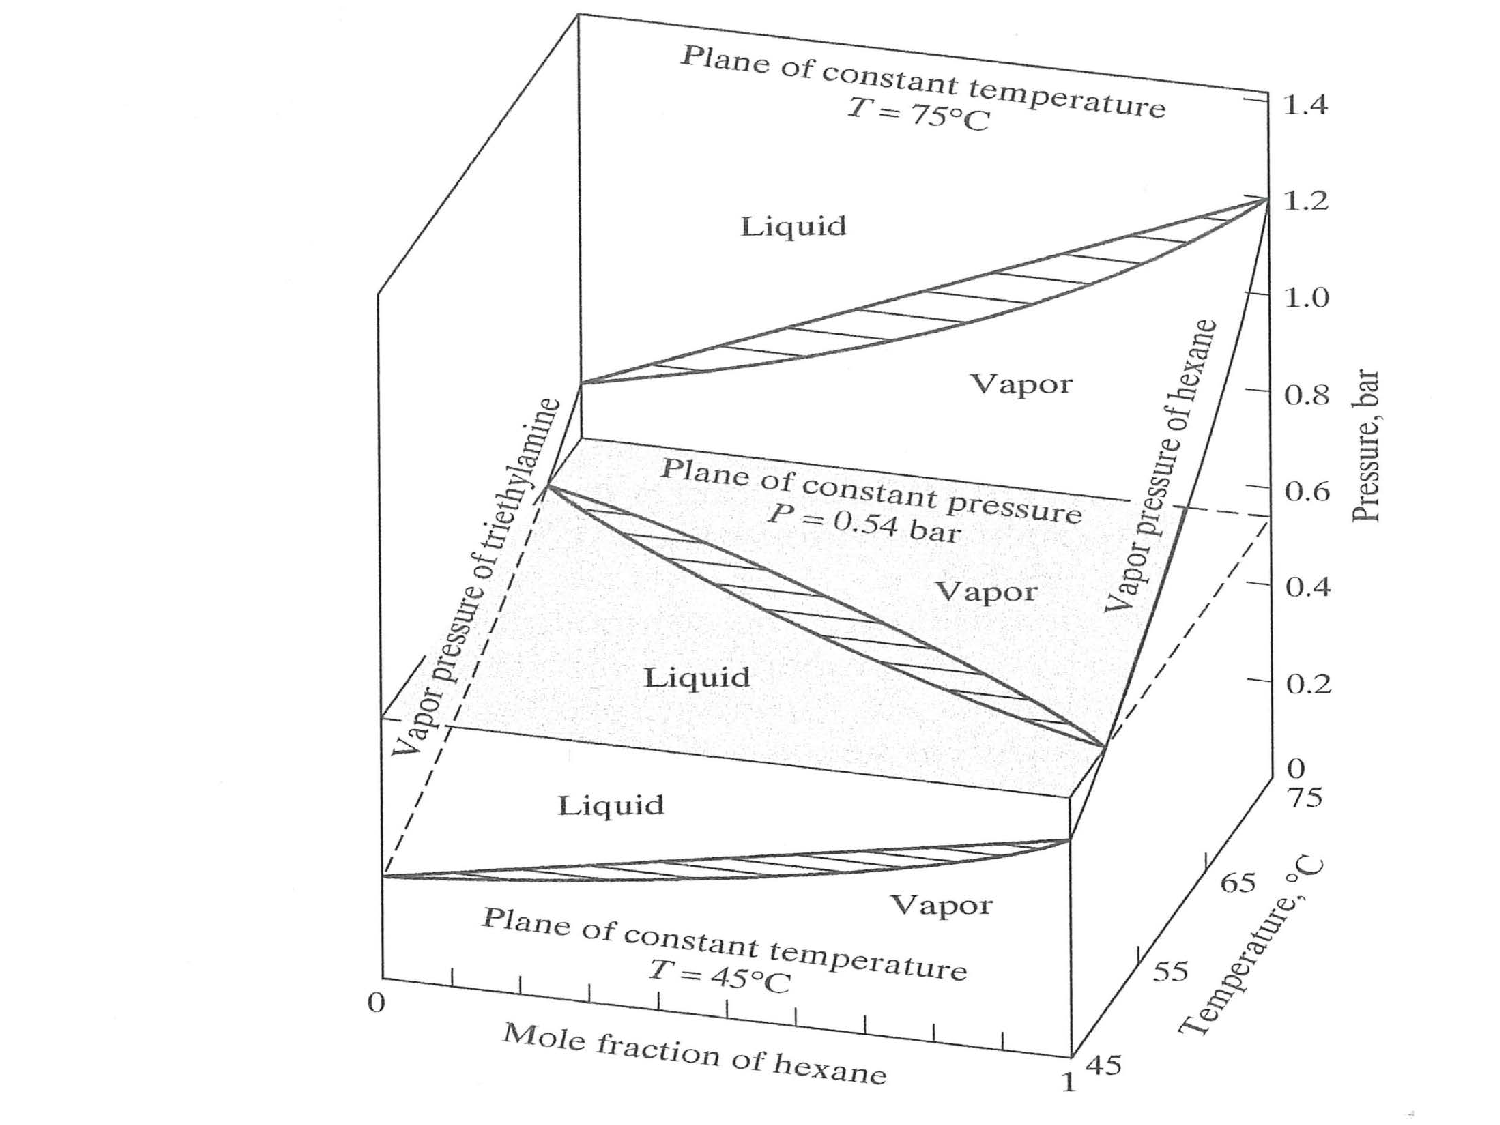
\includegraphics[width=.9\columnwidth,clip]{./../Pics/PTxy_diagram}
           \vspace{-.1cm}\caption{$P-T-xy$ diagram for hexane and triethylamine (extracted from Sandler, 2006).}\label{Mod04Fig01}
         \end{center}
       \end{figure}

In Fig.~\ref{Mod04Fig02}, a generic $P-T-xy$ diagram is shown. Vertical planes parallel to \blue{0-1-R-M-U-0} (\eg plane \blue{E-A-B-D-E}) indicates $P-xy$ diagrams at constant temperature, whereas horizontal planes parallel to \blue{K-J-I-H-K} indicates $T-xy$ diagrams at constant pressure. The (subcooled) liquid region lies \underline{above} the upper surface of the solid (grey) projection, and (superheated) vapour region lies \underline{below} the under surface. The interior of the solid projection between the two surfaces is the region of coexistence of both liquid and vapor phases. 

The $x_{1},y_{1}$ axis is limited to \blue{zero} and \blue{one}, thus at $x_{1}$ (or $y_{1}$) equal to zero, $x_{2}$ (or $y_{2}$) is equal to unity, \ie there is just pure component \blue{2} in solution. Similarly at $x_{1}$ (or $y_{1}$) equal to one, $x_{2}$ (or $y_{2}$) is equal to zero, \ie there is just pure component \blue{1} in solution. The diagram also depicts points \blue{$C_{1}$} and \blue{$C_{2}$} along the vertical planes of $x_{1},y_{1}=0$ and $x_{1},y_{1}=1$, respectively, these two points are the coordinates of the critical conditions $\left(P_{c,1}, P_{c,2}, T_{c,1} \text{ and } T_{c,2}\right)$ of both \underline{pure components}. Critical coordinates for mixtures at various compositions of \blue{1} and \blue{2} lie along a line on the rounded edge of the surface between \blue{$C_{1}$} and \blue{$C_{2}$}.
      \begin{figure}[h] 
         \begin{center}
             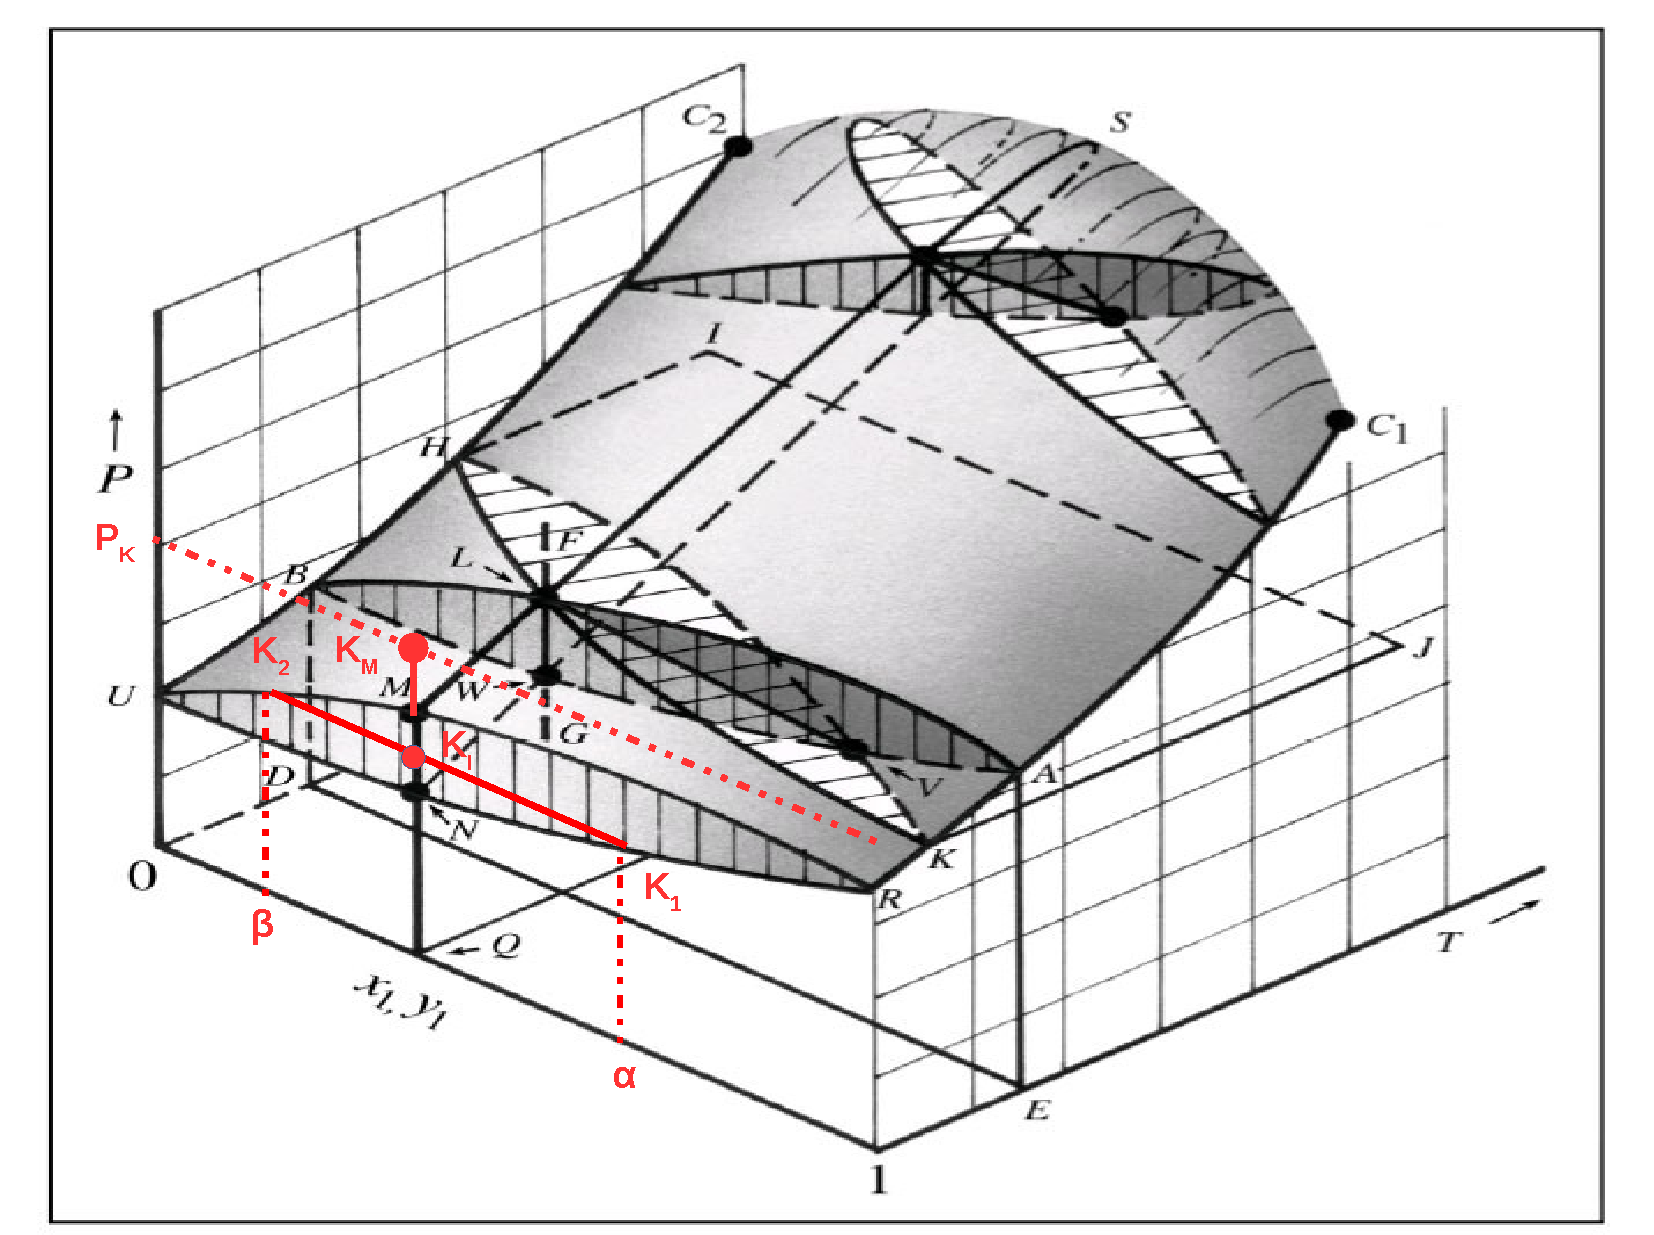
\includegraphics[width=.75\columnwidth,clip]{./Figs/PTxy_Digram} 
             \vspace{-.1cm}\caption{$P-T-xy$ diagram for binary mixtures (extracted from Smith, Van Ness and Abbott, 2000).}\label{Mod04Fig02}
         \end{center}
       \end{figure}
For each constant temperature plane, the upper line of the solid (grey) projection is the \blue{saturated liquid line} whilst the lower line is the \blue{saturated vapour line} (the reader should remember that these lines are also present for pure substances in the $Ts$ and $Ph$ diagrams , Fig.~\ref{Mod03Fig02}).

Compositions of each phase can be obtained from a parallel line linking $x_{1}$ and $y_{1}$. For example, in the `lens' \blue{U-M-R-N-U} contained in the plane \blue{0-U-M-R-1-Q-0}, the vapour phase $\left(\text{with composition }\red{y_{1}=\alpha}\text{ at } \blue{K_{1}}\right)$ is in equilibrium with the liquid phase $\left(\text{with composition }\red{x_{1}=\beta}\text{ at } \blue{K_{2}}\right)$. This parallel line, \blue{$K_{1}-K_{2}$}, is called \underline{tie-line} (Fig.~\ref{Mod04Fig03}b). The intersection of the tie-line with the saturated liquid line is referred as \blue{bubble pressure}, and the intersection with the saturated vapour line is called \blue{dew pressure} (at constant temperature).

$P-T-xy$ diagram, although insightful, is not very practical. Projections of $P-xy$ plane at constant temperature are shown in Fig.~\ref{Mod04Fig03}. Now, let's assume that the fluid of this diagram, Fig.~\ref{Mod04Fig03}(c), is at liquid phase at coordinate \blue{$M$} with composition \blue{$\left(x_{1}=x_{z};y_{1}=0\right)$}. As pressure is reduced along the \blue{$M-S$} line, the first bubble of vapour appears at \blue{$N$}; composition at this coordinate is \blue{$\left(x_{1}=x_{z};y_{1}=y_{BP}\right)$}, and this is called \blue{\it bubble point}. Further reduction of pressure to coordinate \blue{$Q$} (still at constant temperature), the fluid becomes partially vaporised and the composition at this coordinate is given by the {\it tie-line} \blue{$Q_{L}-Q_{V}$} -- \blue{$\left(x_{1}=x_{Q};,y_{1}=y_{Q}\right)$}. 
      \begin{figure}[h]
        \vbox{\hbox{\hspace{-1.cm}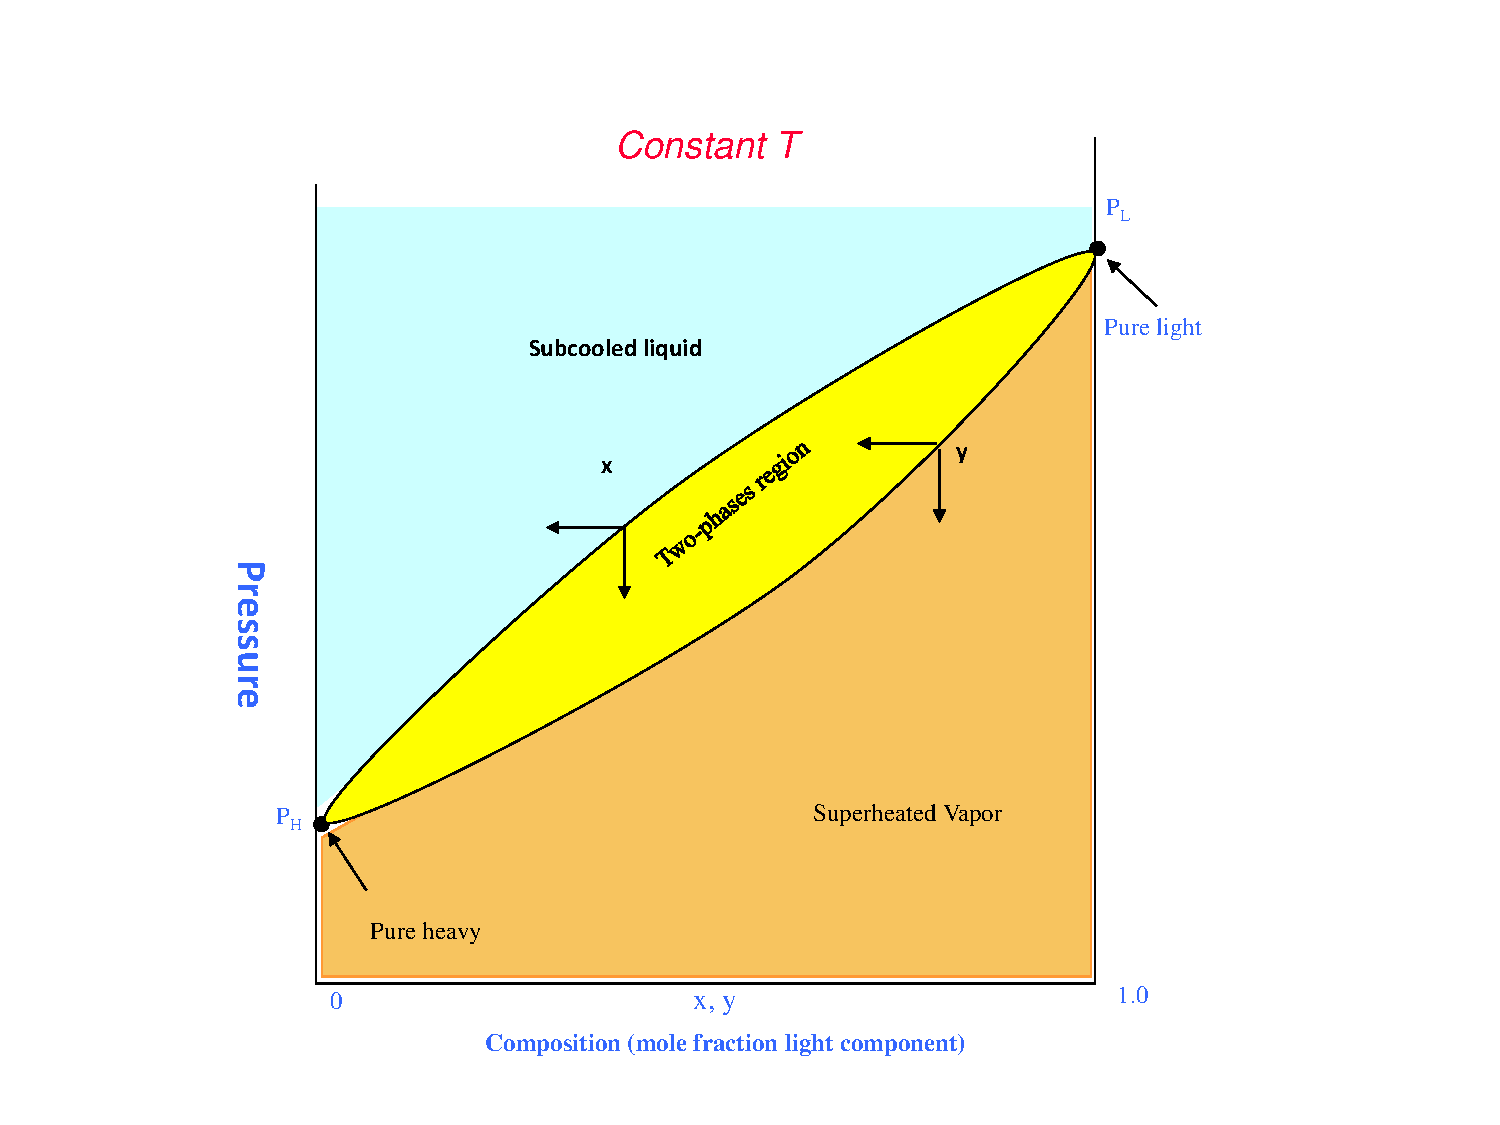
\includegraphics[width=.7\linewidth,clip]{./../Pics/VLE_Pxy_Diagram1}
            \hspace{-4.cm}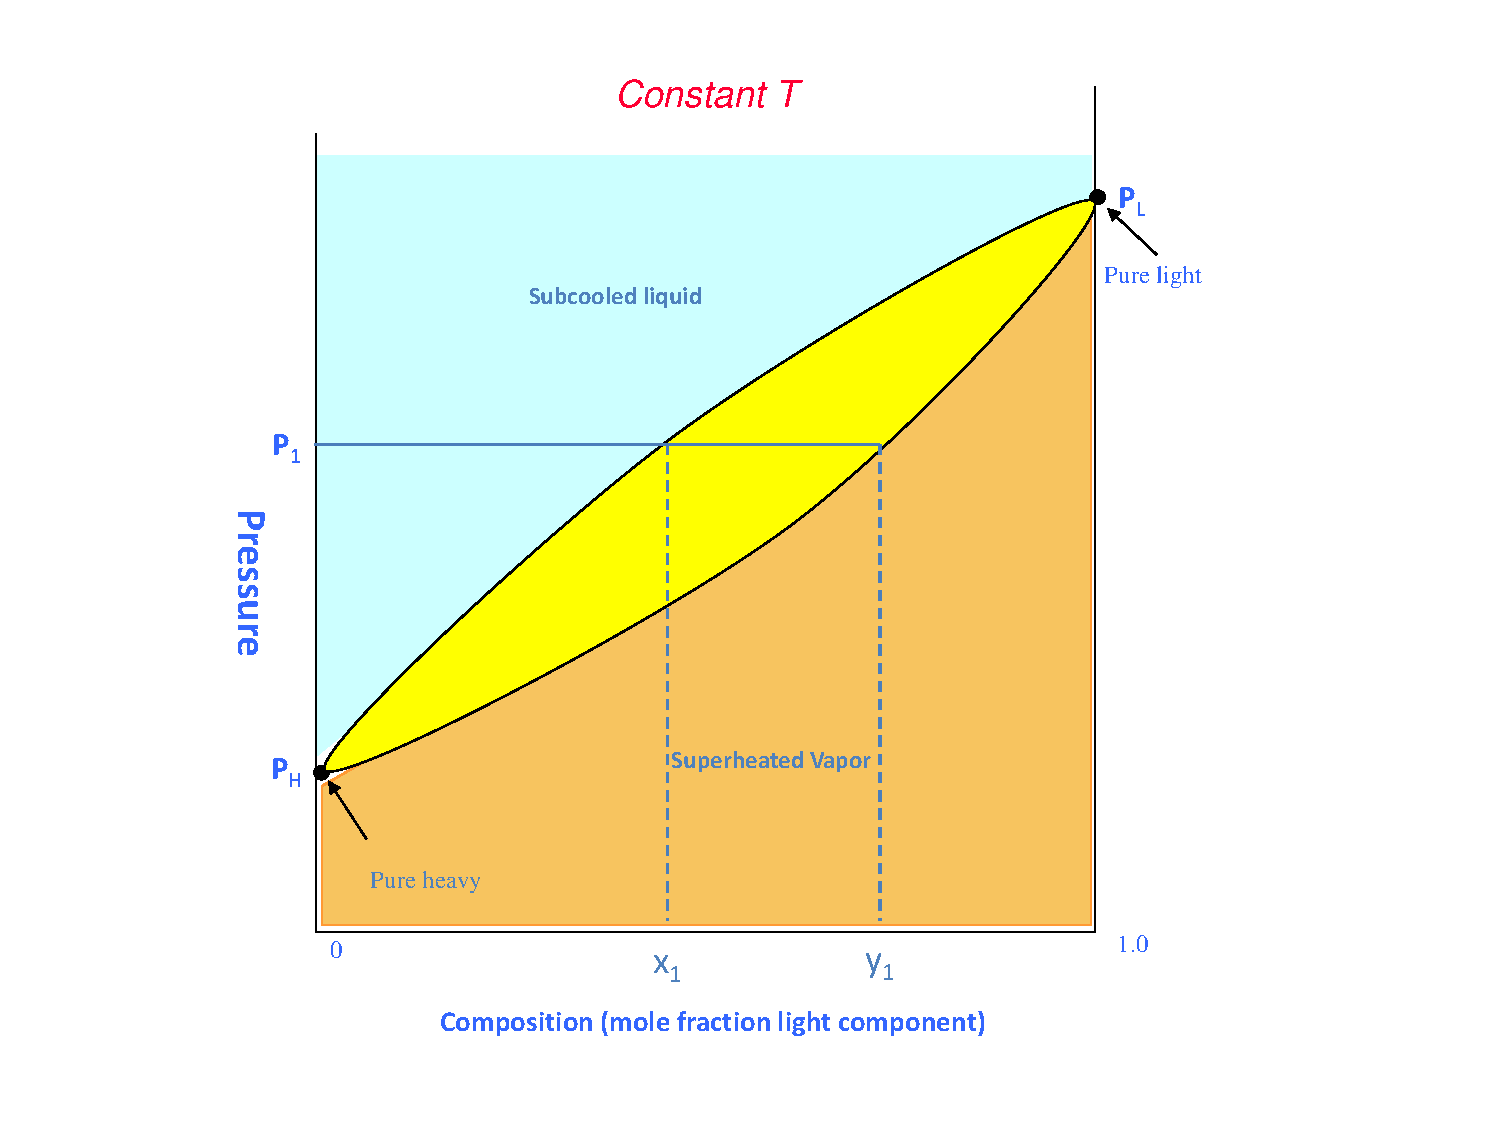
\includegraphics[width=.7\linewidth,clip]{./../Pics/VLE_Pxy_Diagram2}}
          \vspace{-.5cm}
          \hbox{\hspace{4.5cm}(a)\hspace{7cm}(b)}
          \vspace{-.5cm}\hbox{\hspace{3.cm}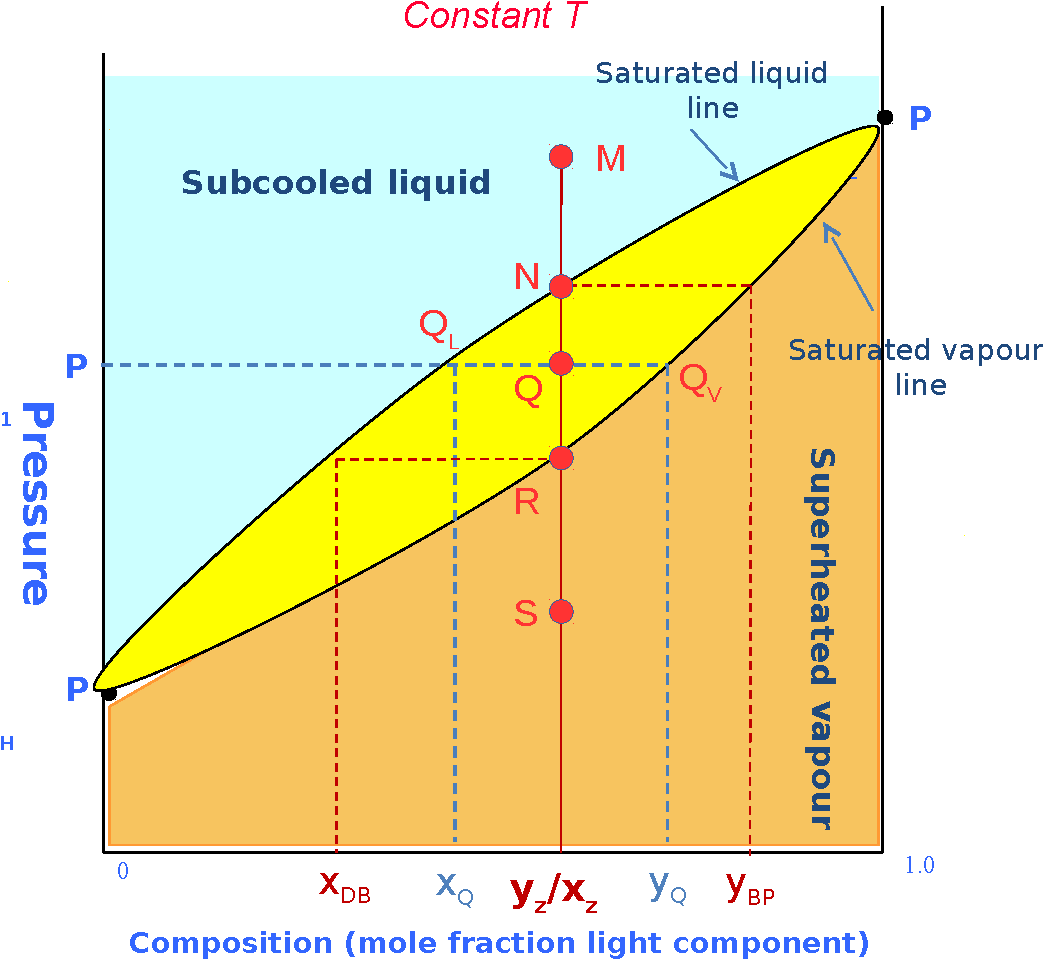
\includegraphics[width=.6\linewidth,clip]{./../Pics/VLE_Pxy_Diagram3b}}
          \vspace{-.1cm}
          \hbox{\hspace{7.5cm}(c)}}
             \vspace{-.1cm}\caption{VLE for binary mixtures: $P-xy$ diagrams at constant temperature.}\label{Mod04Fig03}
      \end{figure}
      
As the pressure is continuously reduced along line \blue{$Q-R$}, more liquid is vaporised until \blue{$R$}, when the last droplet of liquid (dew) is vaporised. This coordinate is called \blue{\it dew point}. The composition at $N$ is \blue{$\left(x_{1}=x_{DB};y_{1}=y_{z}\right)$}. Continued reduction of pressure towards \blue{$S$} leads to (pure) vapour region with composition \blue{$\left(x_{1}=0,y_{1}=y_{z}\right)$}.
     \begin{figure}[h]
        \vbox{\hbox{\hspace{3.cm}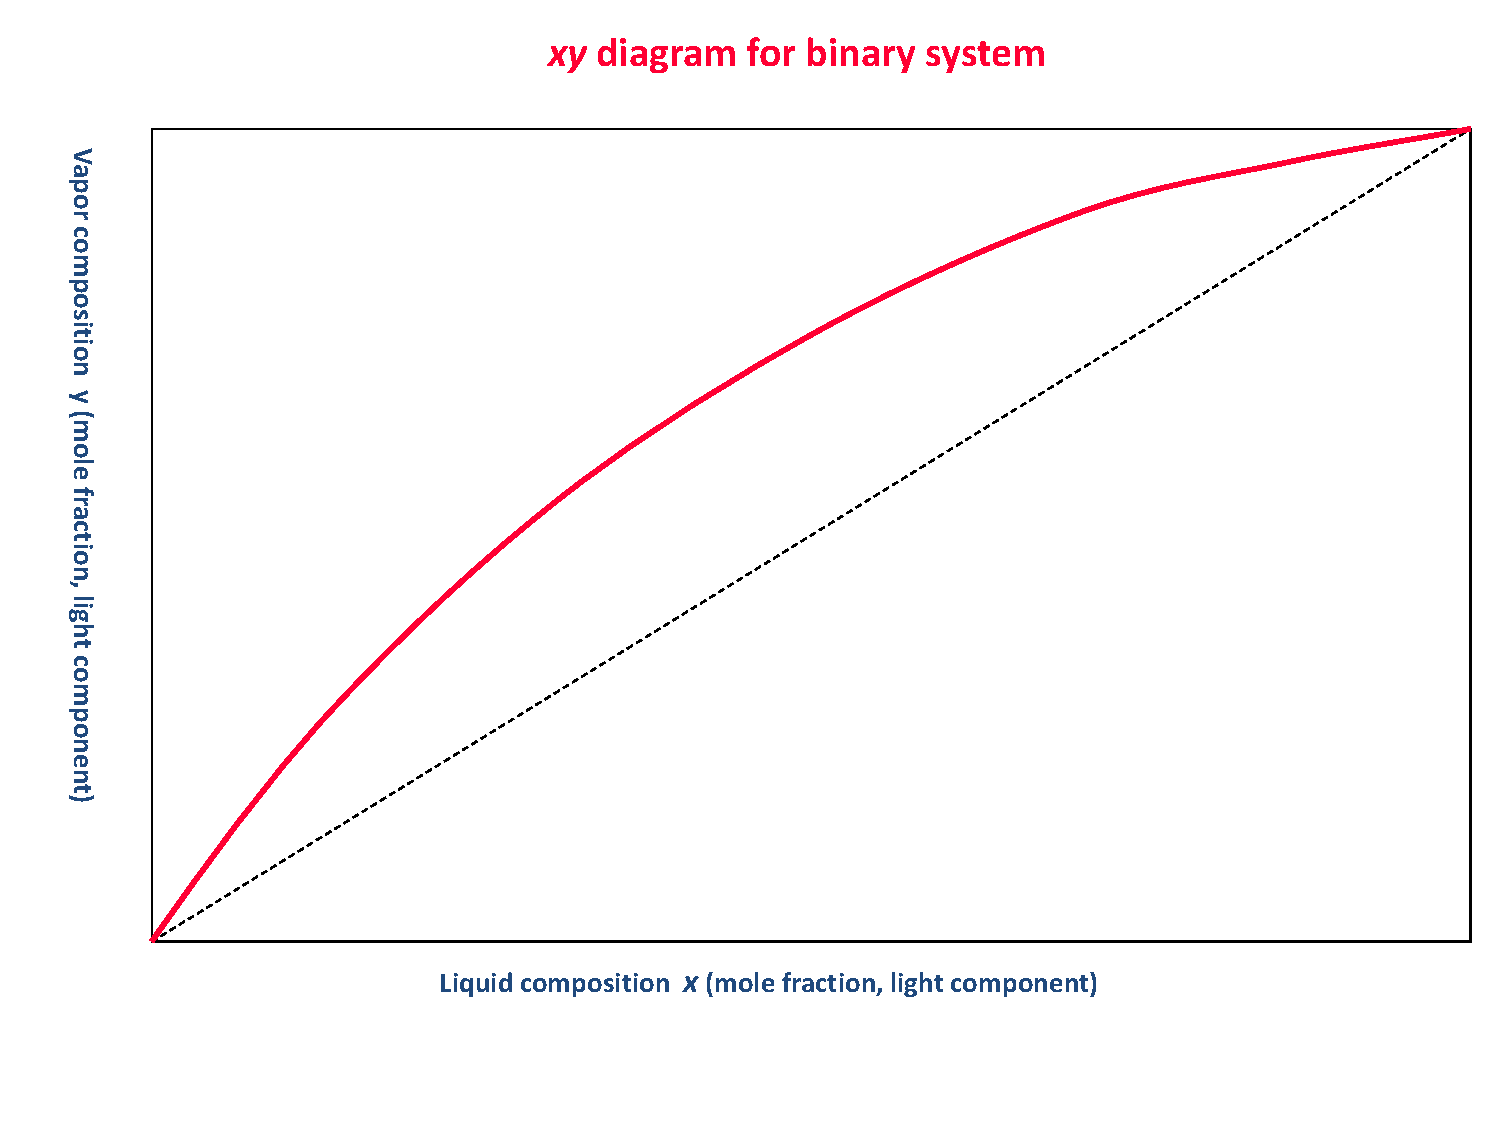
\includegraphics[width=.6\linewidth,clip]{./../Pics/VLE_xy_DiagramIdeal}}
          \vspace{-.5cm}
          \hbox{\hspace{8.cm}(a)}
          \hbox{\hspace{-1.cm}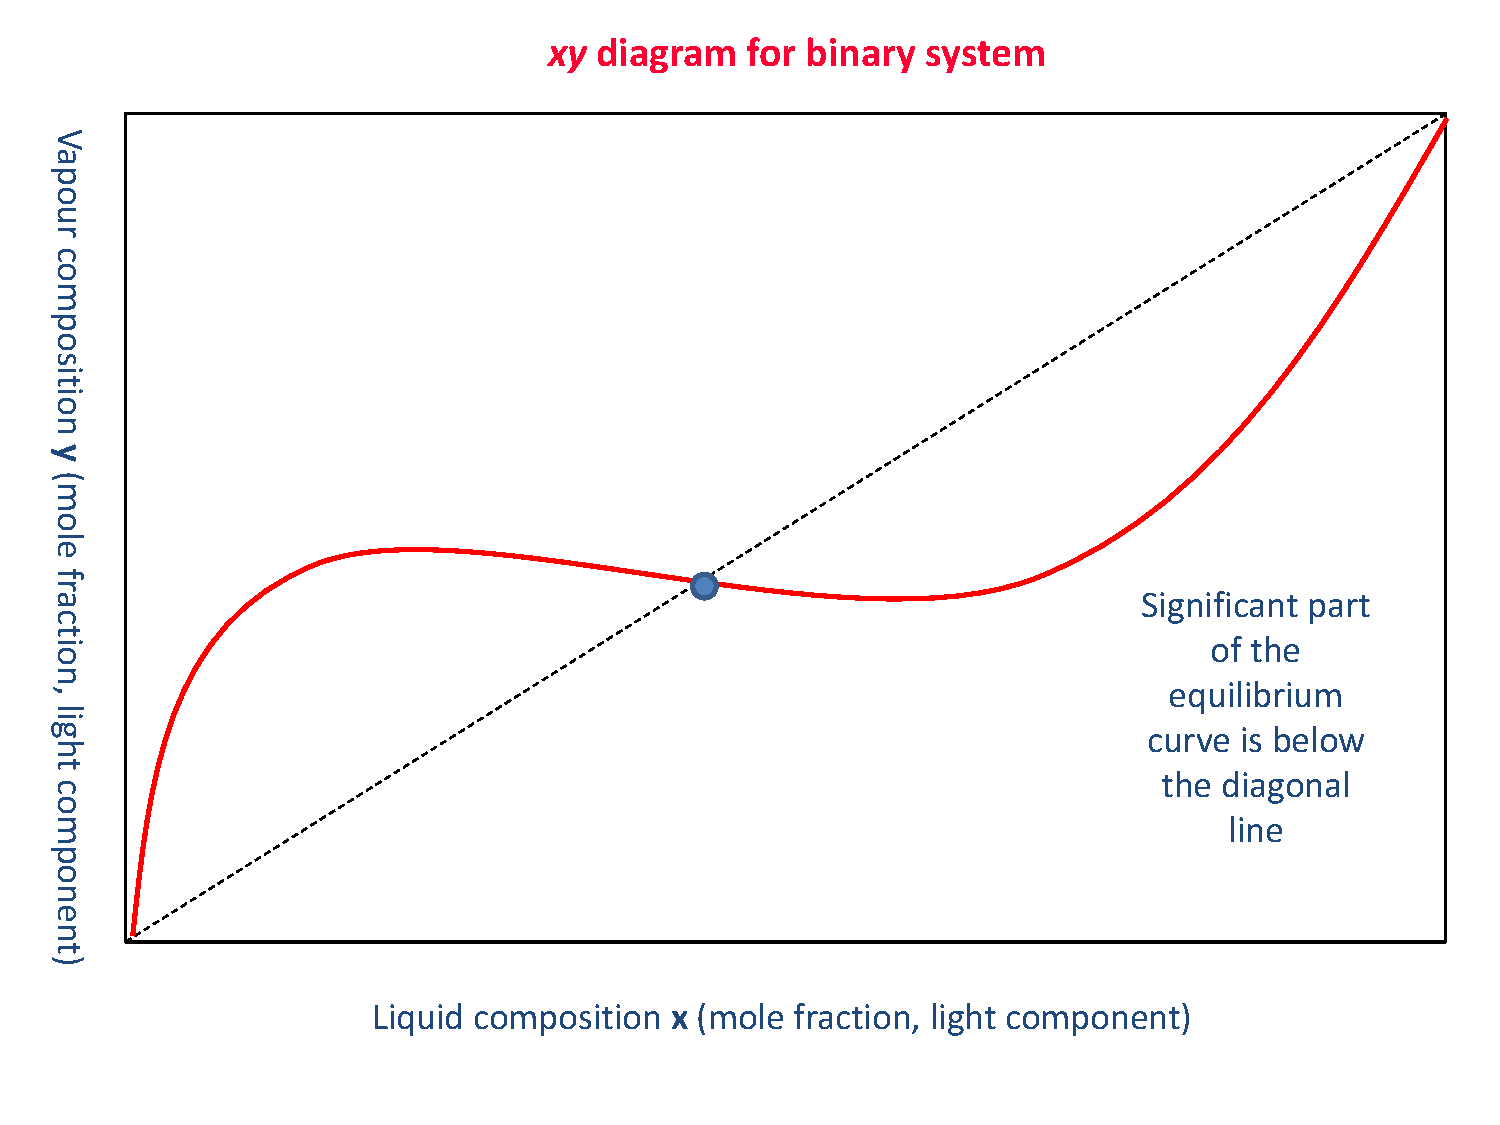
\includegraphics[width=.5\linewidth,clip]{./../Pics/VLE_xy_DiagramNonIdeal1}
            \hspace{-0.cm}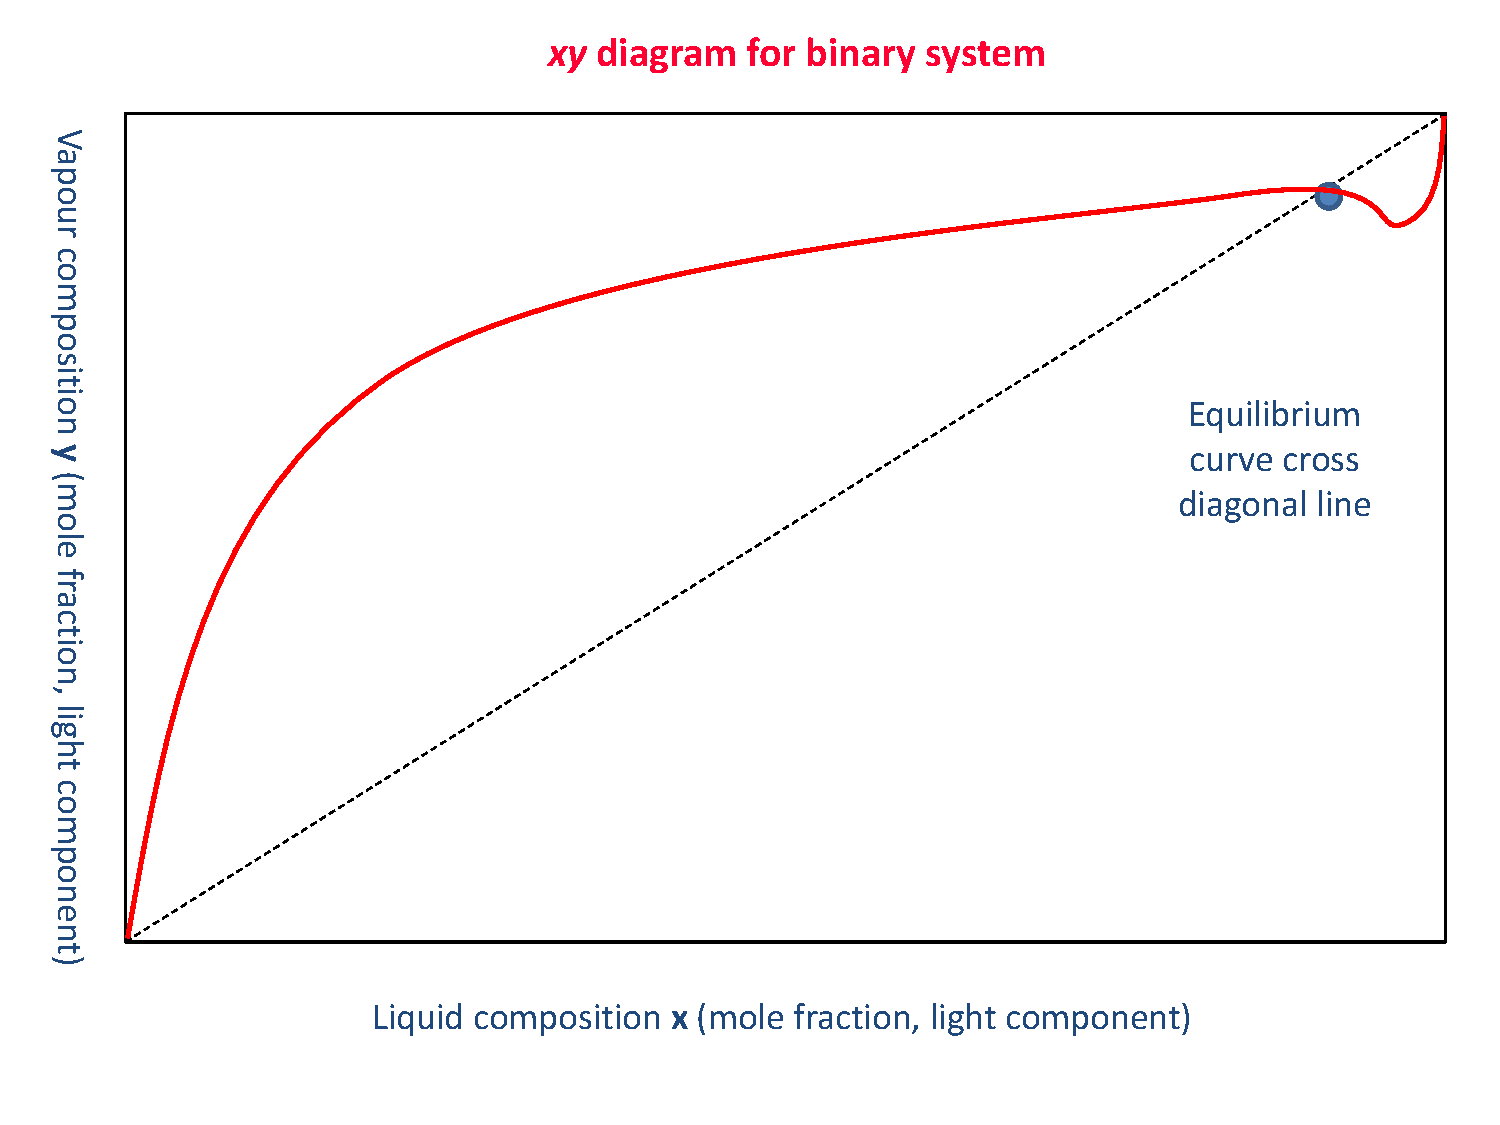
\includegraphics[width=.5\linewidth,clip]{./../Pics/VLE_xy_DiagramNonIdeal2}}
          \vspace{-.5cm}
          \hbox{\hspace{3.5cm}(b)\hspace{7.5cm}(c)}}
          \vspace{-.1cm}\caption{VLE for binary mixtures: $xy$ diagrams at constant pressure of (a) ideal and (b-c) non-ideal solutions.}\label{Mod04Fig04}
      \end{figure}

     Another common phase diagram is the $x-y$, Fig.~\ref{Mod04Fig04}(a), in which either pressure or temperature is kept constant. In this diagram, at constant pressure, there are two curves, the upper curve represents the composition at equilibrium with varying temperature. The straight line represents the equimolar composition, \ie $x_{1}=y_{1}$. However, in several solutions of industrial interest, molecular attractive forces from the heavier component (2) keep molecules of the more volatile component in the liquid solution, constraining its evaporation. This leads into an equilibrium pressure smaller than the expected at the same liquid composition. Such deviation from ideality is called \blue{\it azeotropy}. In practical terms, any component from solutions can often be separated through distillation processes, however azeotropes may lead to vapour-liquid-liquid equilibrium (VLLE) and other separations strategies may need to be used.  
     
%%% SUBSECTION
\subsection{VLE Models: Raoult's Law}\label{Section:04:RaoultsLaw}
  \begin{subequations}
      The diagrams of binary (as well as multi-component) mixtures shown in the previous section are obtained from experiments and introduce a qualitative analysis of the PVT behaviour of solutions. However, classic thermodynamics provides a mathematical framework for systematic correlation, extension, generalisation and interpretation of data.
      For ideal vapour-liquid systems, the \blue{Raoult's law} provides a relation between the compositions of the vapour and liquid phases,
         \begin{shaded}
           \begin{equation}
             P_{i} = y_{i}P = x_{i}P_{i}^{\text{sat}},\;\;\;\forall i\in\left\{1,2,\cdots,\mathcal{C}\right\}\label{Mod04_RaoultLaw} 
           \end{equation}
         \end{shaded}
      $P_{i}=y_{i}P$ in Eqn.~\ref{Mod04_RaoultLaw} is known as \blue{\it partial pressure}, and $P_{i}^{\text{sat}}$ is the saturated pressure (or saturated vapour pressure) of pure species $i$ and was defined in Eqn.~\ref{Mod03_Antoine}. This rather simple relation can only be applied to ideal solutions (for both phases). For a gas mixture to be considered ideal the pressure need to be equal or smaller than atmospheric. There are several relations for ideal gas mixtures, \eg
       \begin{enumerate}[a)]
           \begin{shaded}    
               \item Dalton's Law:
                  \begin{equation}
                      P = \summation[P_{i}]{i=1}{\mathcal{C}} = \summation[y_{i}P]{i=1}{\mathcal{C}}\label{Mod04_DaltonLaw}
                  \end{equation}
           \end{shaded}
           \item Amagat's Law:
              \begin{displaymath}
                  V^{\text{t}} = \summation[V_{i}^{\text{t}}]{i=1}{\mathcal{C}} = \summation[y_{i}V^{\text{t}}]{i=1}{\mathcal{C}}
              \end{displaymath}
           \item Kay's rule for pseudo-critical temperature and pressure:
              \begin{displaymath}
                  T_{c}^{\text{t}} = \summation[y_{i}T_{c,i}]{i=1}{\mathcal{C}},\;\;\text{ and }\;\;P_{c}^{\text{t}} = \summation[y_{i}P_{c,i}]{i=1}{\mathcal{C}}
              \end{displaymath}
       \end{enumerate}
       Liquid solutions are considered ideals if the molecular interaction between the similar species is identical to that between dissimilar species. Thermodynamics of liquid solutions are the focus of Module~\ref{Section:05}.
       
\end{subequations}

%%% SUBSECTION
\subsection{Henry's Law}\label{Section:04:HenryLaw}

A typical application of VLE is when gases are solubilised in liquid solutions, \eg O$_{2}$ in water, CO$_{2}$ in soft drinks, air in the blood stream etc. In these cases, gases have relatively low solubility (mole fraction varying between 10$^{-5}$ to 10$^{-2}$) in liquid solvents. Application of Raoult's law is limited to $P^{\text{sat}}$. If the temperature exceeds the critical temperature, Raoult's law is no longer applicable as $P^{\text{sat}}$ can not be defined. For such cases, a new relation is required that relates compositions in both phases and the pressure,
\begin{shaded}
  \begin{equation}
      P_{i} = y_{i}P = x_{i}\mathcal{H}_{i},\label{Mod04_HenryLaw} 
  \end{equation}
\end{shaded}
\noindent where $\mathcal{H}$ is the Henry's constant obtained experimentally. Values of Henty's contant for several gases dissolved in water at 25$^{\circ}$C is shown in Table~\ref{Mod04_HenryLawTable}
 \begin{table}
  \begin{center}
    \begin{tabular}{l r || l r }
      \hline
       {\bf Gas}    &  ${\bf \mathcal{H}\text{ (bar)}}$ & {\bf Gas}    &  ${\bf \mathcal{H}\text{ (bar)}}$ \\
      \hline
         Acetylene  &   1350                            & He           &  126600 \\
         Air        &   72950                           & H$_{2}$      &  71600  \\
         CO$_{2}$    & 1670                              & H$_{2}$S     & 550 \\
         CO         &  54600                            &  CH$_{4}$    &  41850 \\
         C$_{2}$H$_{6}$ & 30600                          &  N$_{2}$     & 87650  \\
         Ethylene  & 11550                              & O$_{2}$      & 44380 \\
      \hline
    \end{tabular}
    \caption{Henry's constant for gases dissolved in water at 25$^{\circ}$C.}\label{Mod04_HenryLawTable}
  \end{center}
\end{table}

  
%%% SECTION
\section{Industrial Applications: Multi-Component VLE}

%%% SUBSECTION
\subsection{Dew-point and Bubble-point Calculations using Raoult’s Law }

Let's consider a vapour-liquid system containing $\mathcal{C}$ chemical species. From the phase rule the number of degrees of freedom is $\mathcal{C}$ that are $T$, $P$, $x_{i}$ and/or $y_{i}$. Four types of problems are possible:
\begin{center}
   \begin{tabular}{|l c c|}
      \hline 
      $\mathbf{VLE}$ {\bf Problem} & {\bf Specified Variables} &  {\bf Computed Variables} \\  
      \hline
          {\bf Bubble Pressure}        &  $T$ and $x_{i}$           &   $P$ and $y_{i}$          \\
          {\bf Dew Pressure}           &  $T$ and $y_{i}$           &   $P$ and $x_{i}$          \\
          {\bf Bubble Temperature}     &  $P$ and $x_{i}$           &   $T$ and $y_{i}$          \\
          {\bf Dew Temperature}        &  $P$ and $y_{i}$           &   $T$ and $x_{i}$          \\     
      \hline
   \end{tabular}
\end{center}
Such problems are calculated using three relations:
\begin{displaymath}
    P_{i} = y_{i}P = x_{i}P_{i}^{\text{sat}}, \;\;\; \summation[x_{i}]{i=1}{\mathcal{C}} = 1, \;\;\text{ and }\;\; \summation[y_{i}]{i=1}{\mathcal{C}} = 1,
\end{displaymath}
bearing in mind that $P_{i}^{\text{sat}}$ is expressed as a function of $T$. Thus,
\begin{enumerate}[a)]
    \item Bubble pressure: Given $T$ and $x_{i}$ $\left(\text{with }i=1,\cdots,\mathcal{C}\right)$, find $P$ that solves,
        \begin{displaymath}
           \summation[y_{i}]{i=1}{\mathcal{C}} = 1 \;\;\Longrightarrow\;\; \summation[\frc{x_{i}P_{i}^{\text{sat}}}{P}]{i=1}{\mathcal{C}} = 1,
        \end{displaymath}
        and then calculate $y_{i}= \frc{x_{i}P_{i}^{\text{sat}}}{P}$.
        
    \item Bubble temperature: Given $P$ and $x_{i}$ $\left(\text{with }i=1,\cdots,\mathcal{C}\right)$, find $T$ that solves,
        \begin{displaymath}
           \summation[y_{i}]{i=1}{\mathcal{C}} = 1 \;\;\Longrightarrow\;\; \summation[\frc{x_{i}P_{i}^{\text{sat}}}{P}]{i=1}{\mathcal{C}} = 1,
        \end{displaymath}
        and then calculate $y_{i}= \frc{x_{i}P_{i}^{\text{sat}}}{P}$.
      
    \item Dew pressure: Given $T$ and $y_{i}$ $\left(\text{with }i=1,\cdots,\mathcal{C}\right)$, find $P$ that solves,
        \begin{displaymath}
           \summation[x_{i}]{i=1}{\mathcal{C}} = 1 \;\;\Longrightarrow\;\; \summation[\frc{y_{i}P}{P_{i}^{\text{sat}}}]{i=1}{\mathcal{C}} = 1,
        \end{displaymath}
        and then calculate $y_{i}= \frc{x_{i}P_{i}^{\text{sat}}}{P}$.
      
    \item Dew temperature: Given $P$ and $y_{i}$ $\left(\text{with }i=1,\cdots,\mathcal{C}\right)$, find $T$ that solves,
        \begin{displaymath}
           \summation[x_{i}]{i=1}{\mathcal{C}} = 1 \;\;\Longrightarrow\;\; \summation[\frc{y_{i}P}{P_{i}^{\text{sat}}}]{i=1}{\mathcal{C}} = 1,
        \end{displaymath}
        and then calculate $y_{i}= \frc{x_{i}P_{i}^{\text{sat}}}{P}$.
\end{enumerate}


%%% SUBSECTION
\subsection{K-Value Correlations for Hydrocarbon Systems}

As discussed in Modules~\ref{Section:02}-~\ref{Section:03}, cubic equations of state are often used to describe the PVT behaviour of vapour and liquid phases of pure chemical species and mixtures. Although the use of cubic EOS is widely spread over the chemical industry, applicability to liquid phase is still limited. Several alternatives have been proposed and developed over the past 50 years, one of them, mostly used in petroleum and petrochemical industry for hydrocarbons, is called {\it K-value correlation}. $K$ is defined as
\begin{shaded}
   \begin{equation}
      K_{i} = \frc{P_{i}^{\text{sat}}}{P} = \frc{y_{i}}{x_{i}}.\label{Mod04_KValue}
   \end{equation}
\end{shaded}
Values for $K_{i}$ are tabulated for a large number of hydrocarbons at several pressure and temperature conditions and can be found in any chemical engineering handbook as part of \blue{DePriester chart} (Fig.~\ref{Mod04Fig05}).
  \begin{figure}[h]
     \begin{center}
         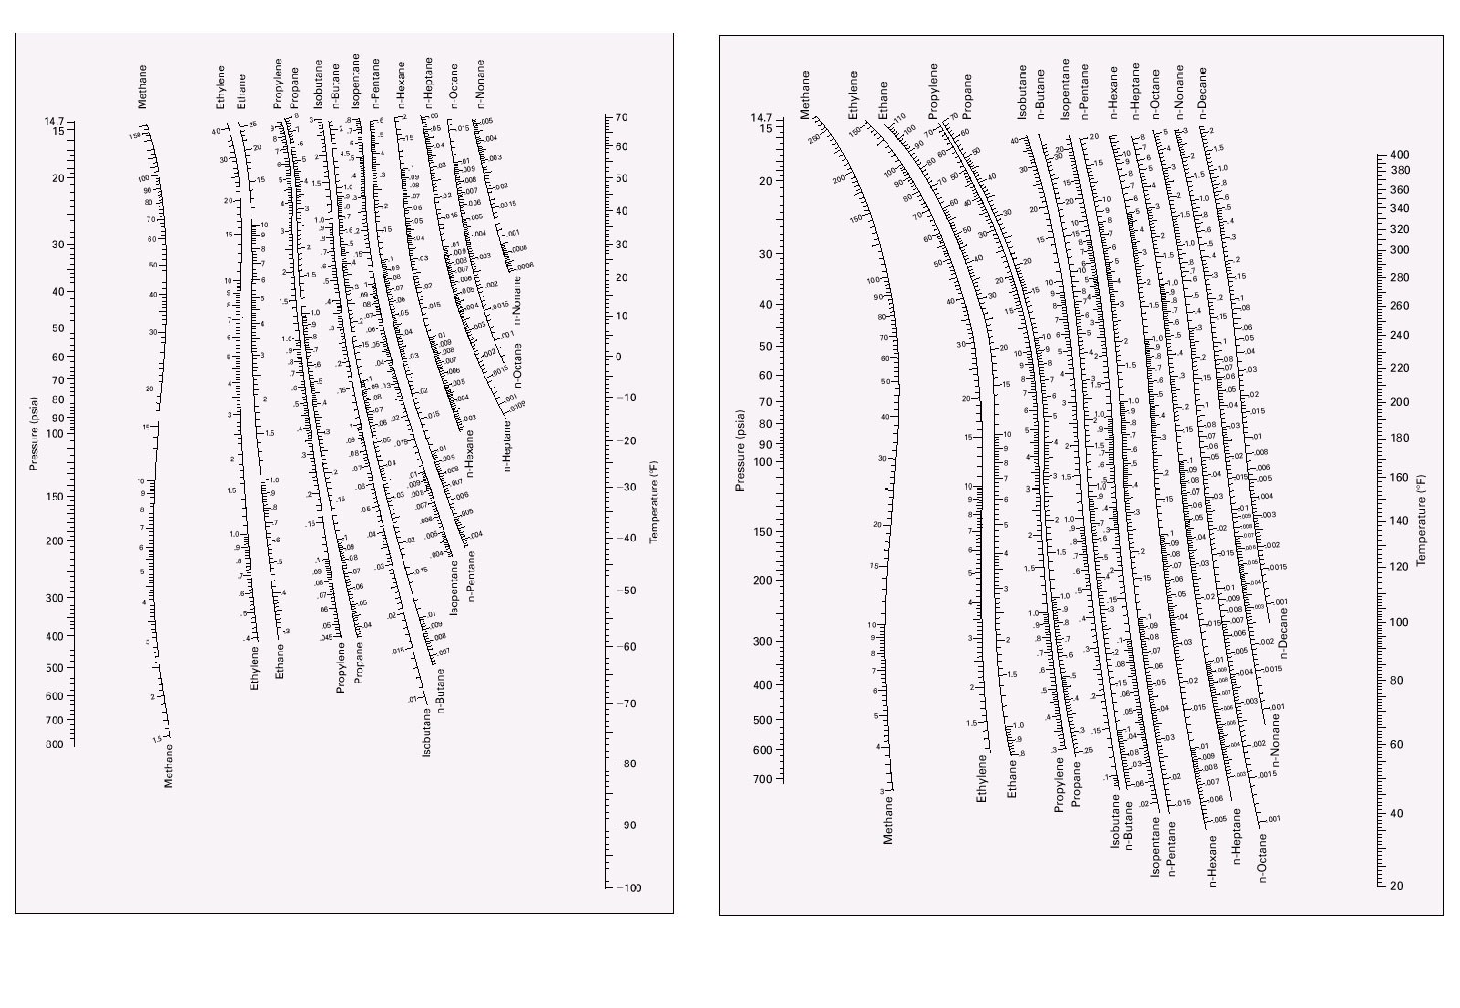
\includegraphics[width=1.\linewidth,clip]{./Figs/DePriesterCharts}
     \end{center}
     \caption{DePriester chart for several hydrocarbons (extracted from Smith, Van Ness and Abbott, 2000).}\label{Mod04Fig05}
  \end{figure}


%%% SUBSECTION
\subsection{Flash Distillation}\label{Section:04:FlashDistillation}

Flash distillation is a common process in chemical industry to obtain solutions with the required enrichment from a feed-stock. Figure~\ref{Mod04Fig06} shows a schematic of this process, where a liquid stream (\ie with pressure equal to or larger than its bubble point pressure) with molar fraction $F$ and overall composition $z_{i}$ is injected into a separation vessel through a pressure reduction valve. The sudden reduction in pressure leads to partial evaporation (\ie {\it flash}) of the liquid feed resulting in the formation of a vapour and a liquid stream. Vapour and Liquid streams have molar fraction $V$ and $L$, respectively, with compositions of $y_{i}$ and $x_{i}$. 
  \begin{figure}[h]
     \begin{center}
         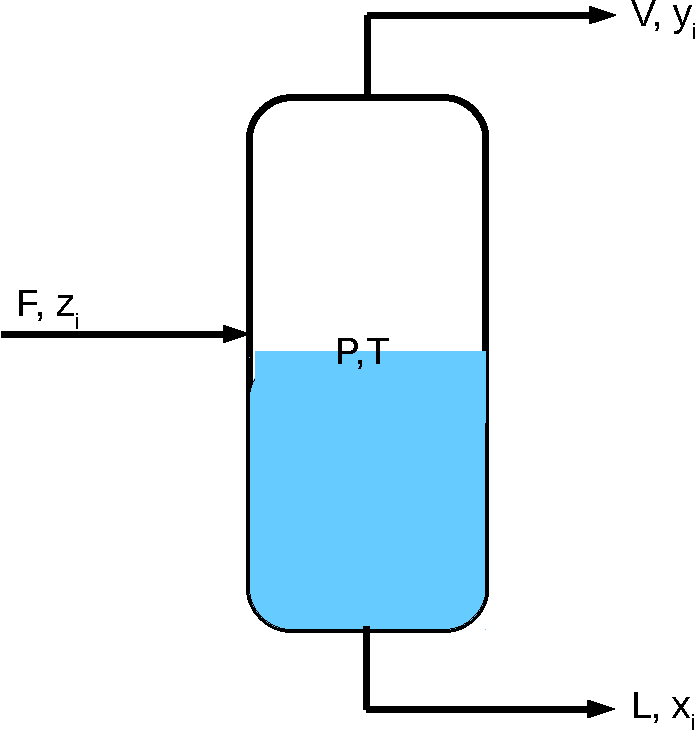
\includegraphics[width=.7\linewidth,clip]{./Figs/FlashDistillation}
     \end{center}
     \caption{Schematic of a flash distillation process.}\label{Mod04Fig06}
  \end{figure}
        
      The overall mass balance of the system is
         \begin{displaymath}
             F = V + L,
         \end{displaymath}
         for convenience, $F$ is assumed equal to unity, $F=1$. Similarly, the mass balance for each component $i$ is
         \begin{displaymath}
            z_{i} = x_{i}L + y_{i}V = x_{i}\left(1-V\right) + y_{i}V.
         \end{displaymath}
         Replacing $x_{i} = \frc{y_{i}}{K_{i}}$,
         \begin{displaymath}
           z_{i} = \frc{y_{i}}{K_{i}}\left(1-V\right) + y_{i}V \;\;\Longrightarrow \;\;y_{i} = \frc{z_{i}K_{i}}{1+V\left(K_{1}-1\right)}. 
         \end{displaymath}
         As $\summation[y_{i}]{i=1}{\mathcal{C}} = 1$,
         \begin{shaded}
           \begin{equation}
              \summation[\frc{z_{i}K_{i}}{1+V\left(K_{i}-1\right)}]{i=1}{\mathcal{C}} = 1.\label{Mod04_FlashEquation} 
           \end{equation}
         \end{shaded}
         Solving a $P-T$ flash problem is to \underline{find $V$} that satisfies Eqn.~\ref{Mod04_FlashEquation}.
      
\clearpage

%%% SECTION
\section{Examples}

\begin{enumerate}[1)] 
%%%
%%% EXAMPLE
%%%
   \item\label{Mod04Ex01} Assuming a mixture of n-pentane $\left(nC_{5}\right)$ and n-heptane $\left(nC_{7}\right)$ is ideal, draw vapour-liquid $x_{5}\times y_{5}$ and $P-x_{5}y_{5}$ equilibrium diagrams for this mixtures at constant temperature of 50$^{\circ}$C. Given $P^{\text{sat}}$ relation,
    \begin{displaymath}
      \ln{P_{i}^{\text{sat}}} = A_{i} - \frc{B_{i}}{RT}
    \end{displaymath}
    with $A_{nC_{5}}=10.422$, $A_{nC_{7}}=11.431$, $B_{nC_{5}}=26799 \text{ J.mol}^{-1}$ and $B_{nC_{7}}=35200 \text{ J.mol}^{-1}$. Also [$P$] = bar and [$T$] = K.

% SOLUTION
 \noindent{\bf Solution:} At $T=$50$^{\circ}$C = 323.15 K, vapour saturated pressures for $nC_{5}$ and $nC_{7}$ (for short notation, let's use 5 and 7 as $nC_{5}$ and $nC_{7}$, respectively) are
           \begin{displaymath}
              P_{5}^{\text{sat}} = 1.5639\text{ bar}\;\;\text{ and }\;\;P_{7}^{\text{sat}} = 0.1881\text{ bar}.
           \end{displaymath}
           In order to calculate the equilibrium pressure at each liquid $nC_{5}$ composition, $x_{5}$,
           \begin{eqnarray}
               && P_{i} = x_{i}P_{i}^{\text{sat}} \;\;\Longleftrightarrow \;\; P = \summation[P_{i}]{i=1}{\mathcal{C}} = \summation[x_{i}P_{i}^{\text{sat}}]{i=1}{\mathcal{C}} \nonumber \\
               && P = x_{5}P_{5}^{\text{sat}} + x_{7}P_{7}^{\text{sat}} = x_{5}P_{5}^{\text{sat}} + \left(1-x_{5}\right)P_{7}^{\text{sat}} \nonumber 
           \end{eqnarray}
           And for vapour composition (Raoult's law),
           \begin{displaymath}
               y_{i} P = x_{i}P_{i}^{\text{sat}}  \;\;\Longleftrightarrow \;\; y_{5} = \frc{x_{5}P_{5}^{\text{sat}}}{P},
           \end{displaymath}
           replacing pressure, $P$, from the previous equation
           \begin{displaymath}
               y_{5} = \frc{x_{5}P_{5}^{\text{sat}}}{x_{5}P_{5}^{\text{sat}} + \left(1-x_{5}\right)P_{7}^{\text{sat}}}.
           \end{displaymath}
           The $x_{5} \times y_{5}$ diagram may be plot by giving values to $0.0\leq x_{5} \leq 1.0$ and calculating $x_{5}$ through the equation above.

           The $P-x_{5}y_{5}$ diagram may be plot using the relations,
           \begin{displaymath}
               y_{5} = \frc{x_{5}P_{5}^{\text{sat}}}{P}\;\;\;\text{ and }\;\;\; P = x_{5}P_{5}^{\text{sat}} + \left(1-x_{5}\right)P_{7}^{\text{sat}} \;\Longrightarrow\; x_{5} = \frc{P-P_{7}^{\text{sat}}}{P_{5}^{\text{sat}}-P_{7}^{\text{sat}}}.
           \end{displaymath}
           Thus, given values for $P_{7}^{\text{sat}}\leq P \leq P_{5}^{\text{sat}}$ $\Rightarrow$ Calculate $x_{5}$  $\Rightarrow$ Calculate $y_{5}$.
           
      \begin{figure}[h]
         \vbox{
             \hbox{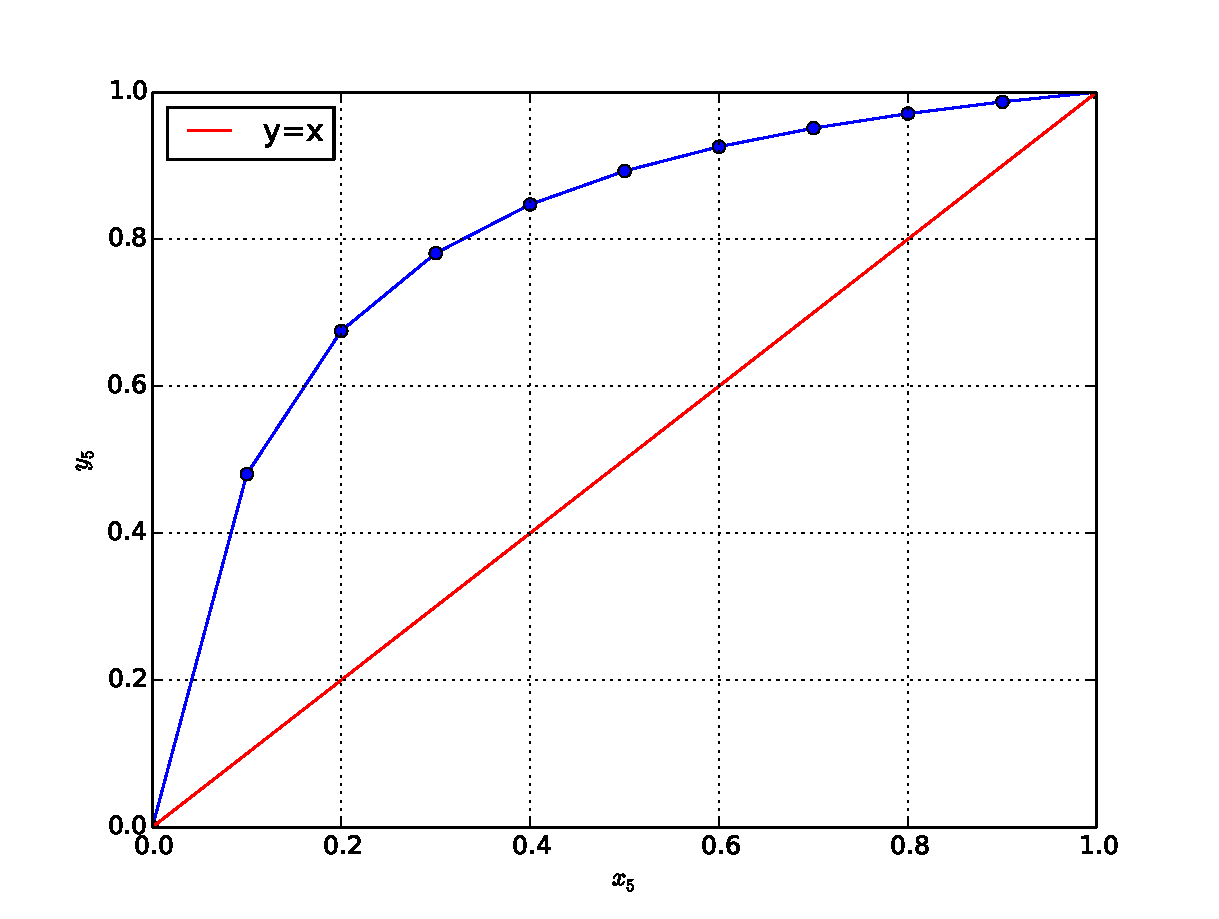
\includegraphics[width=.5\linewidth,clip]{./Figs/Mod4Ex1}
                   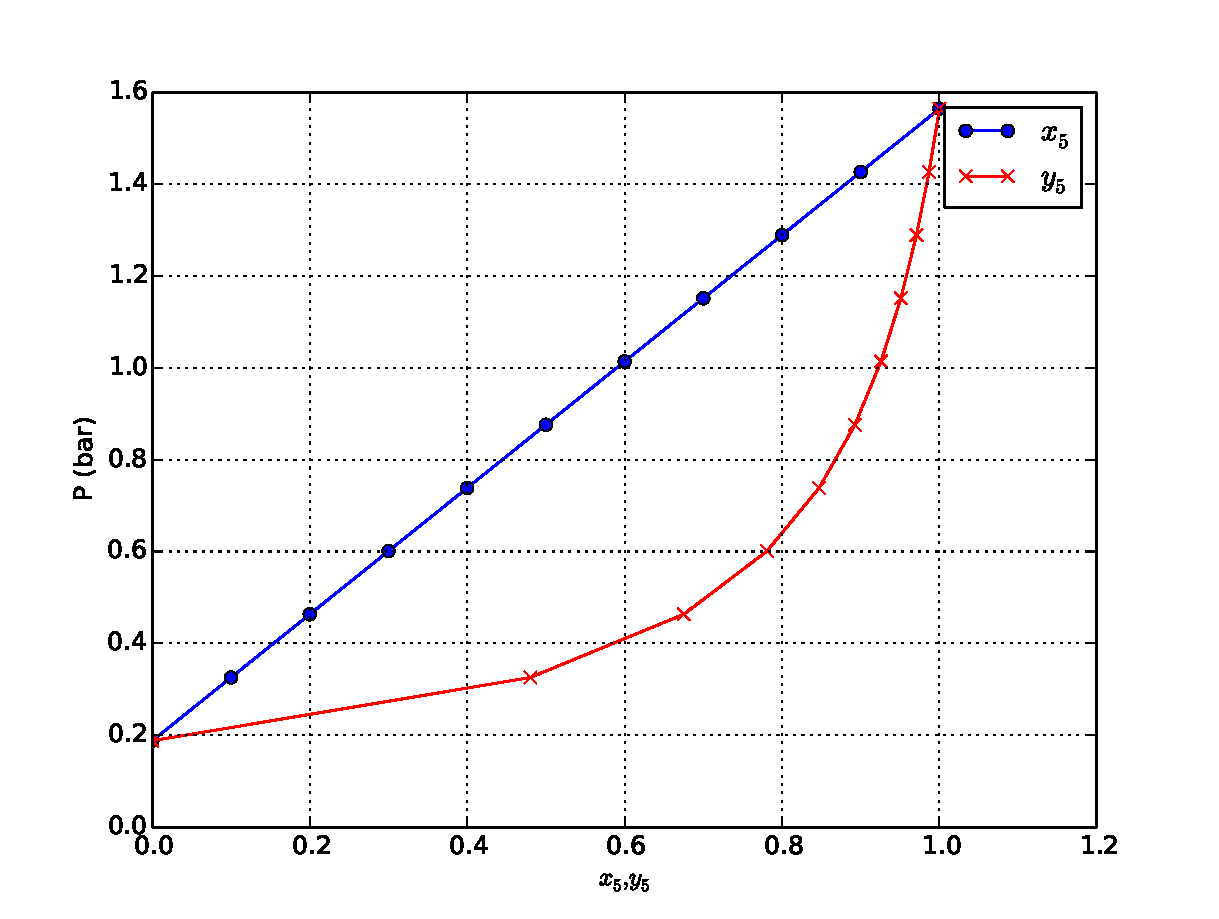
\includegraphics[width=.5\linewidth,clip]{./Figs/Mod4Ex1b}}}
         \caption{Example~\ref{Mod04Ex01}}
      \end{figure}
\clearpage
 % 
%%%
%%% EXAMPLE
%%%
   \item\label{Mod04Ex02} Assuming a mixture of n-pentane $\left(nC_{5}\right)$ and n-heptane $\left(nC_{7}\right)$ is ideal, draw vapour-liquid $x_{5}\times y_{5}$ and $T-x_{5}y_{5}$ equilibrium diagrams for this mixtures at constant pressure of 1.013 bar. Given $P^{\text{sat}}$ relation,
    \begin{displaymath}
      \ln{P_{i}^{\text{sat}}} = A_{i} - \frc{B_{i}}{RT}
    \end{displaymath}
    with $A_{nC_{5}}=10.422$, $A_{nC_{7}}=11.431$, $B_{nC_{5}}=26799 \text{ J.mol}^{-1}$ and $B_{nC_{7}}=35200 \text{ J.mol}^{-1}$. Also [$P$] = bar and [$T$] = K.

% SOLUTION
 \noindent{\bf Solution:} In this problem, equilibrium temperature and compositions are not known, thus
          \begin{displaymath}
              P = x_{5}P_{5}^{\text{sat}} + x_{7}P_{7}^{\text{sat}} = x_{5}P_{5}^{\text{sat}} + \left(1 - x_{5}\right)P_{7}^{\text{sat}} = 1.013\text{ bar},
          \end{displaymath}
          where $P_{i}^{\text{sat}}$ is non-linear function of the temperature $T$, \ie
          \begin{displaymath}
              P = x_{5}\exp{\left(A_{5} - \frc{B_{5}}{RT}\right)} + \left(1 - x_{5}\right)\exp{\left(A_{7} - \frc{B_{7}}{RT}\right)}.
          \end{displaymath}
          This equation has 2 unknowns, $x_{5}$ and $T$, however we know that $0.0\leq x_{5} \leq 1.0$, thus we can give values on this range $\Rightarrow$ calculate $T$  $\Rightarrow$  obtain $y_{5}$.
          \begin{center}
              \begin{tabular}{ c c c }
                  $\mathbf{x_{5}}$ & $\mathbf{T}${\bf(K)}  & $\mathbf{y_{5}}$ \\
                    0.0000          & 370.80                & 0.0000   \\
                    0.1000          & 357.80                & 0.4050   \\
                    0.2000          & 347.73                & 0.6249   \\
                    0.3000          & 339.73                & 0.7535   \\
                    0.4000          & 333.21                & 0.8345   \\
                    0.5000          & 327.77                & 0.8881   \\
                    0.6000          & 323.13                & 0.9257   \\
                    0.7000          & 319.12                & 0.9528   \\
                    0.8000          & 315.60                & 0.9728   \\
                    0.9000          & 312.47                & 0.9881   \\
                    1.0000          & 309.67                & 1.0000   
              \end{tabular}
           \end{center}
           
      \begin{figure}[h]
         \vbox{
             \hbox{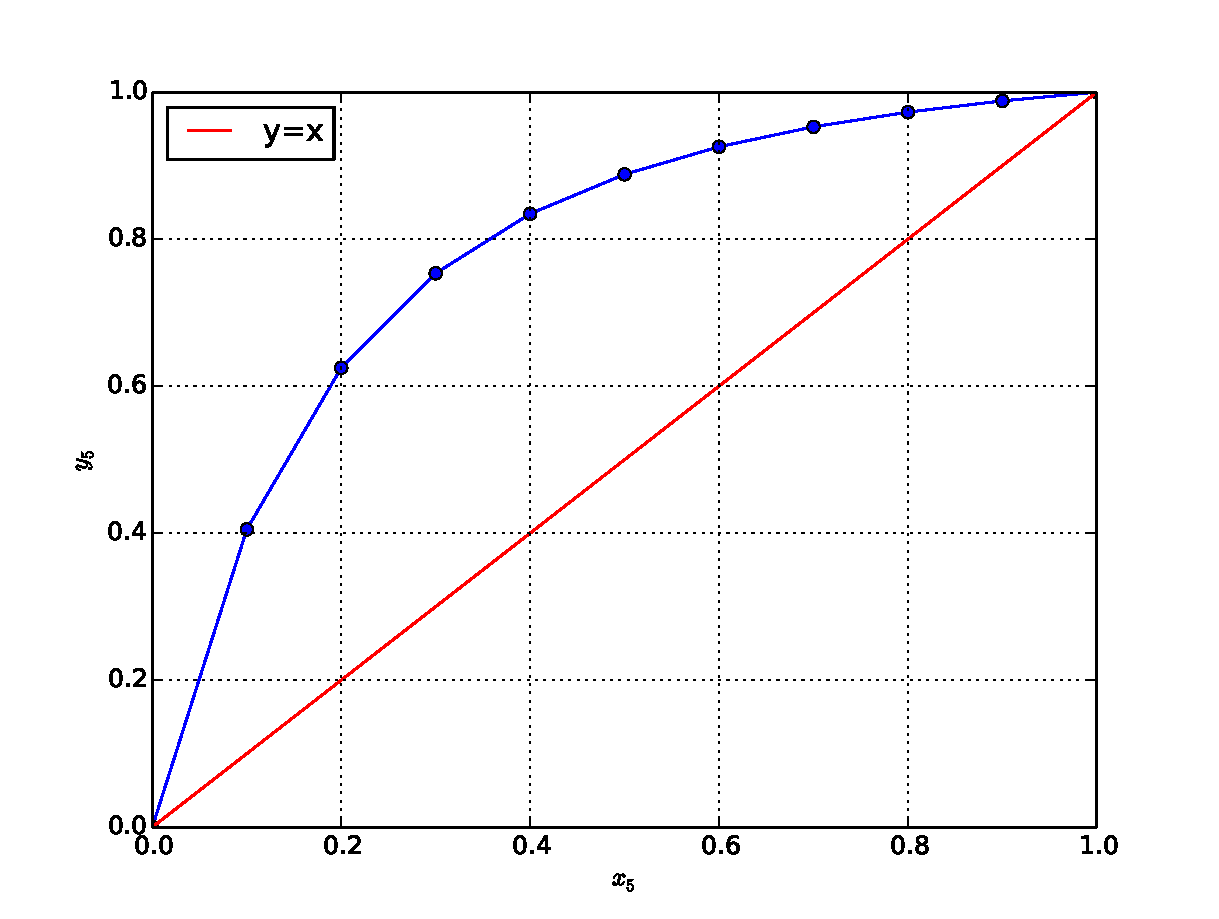
\includegraphics[width=.5\linewidth,clip]{./Figs/Mod4Ex2a}
                   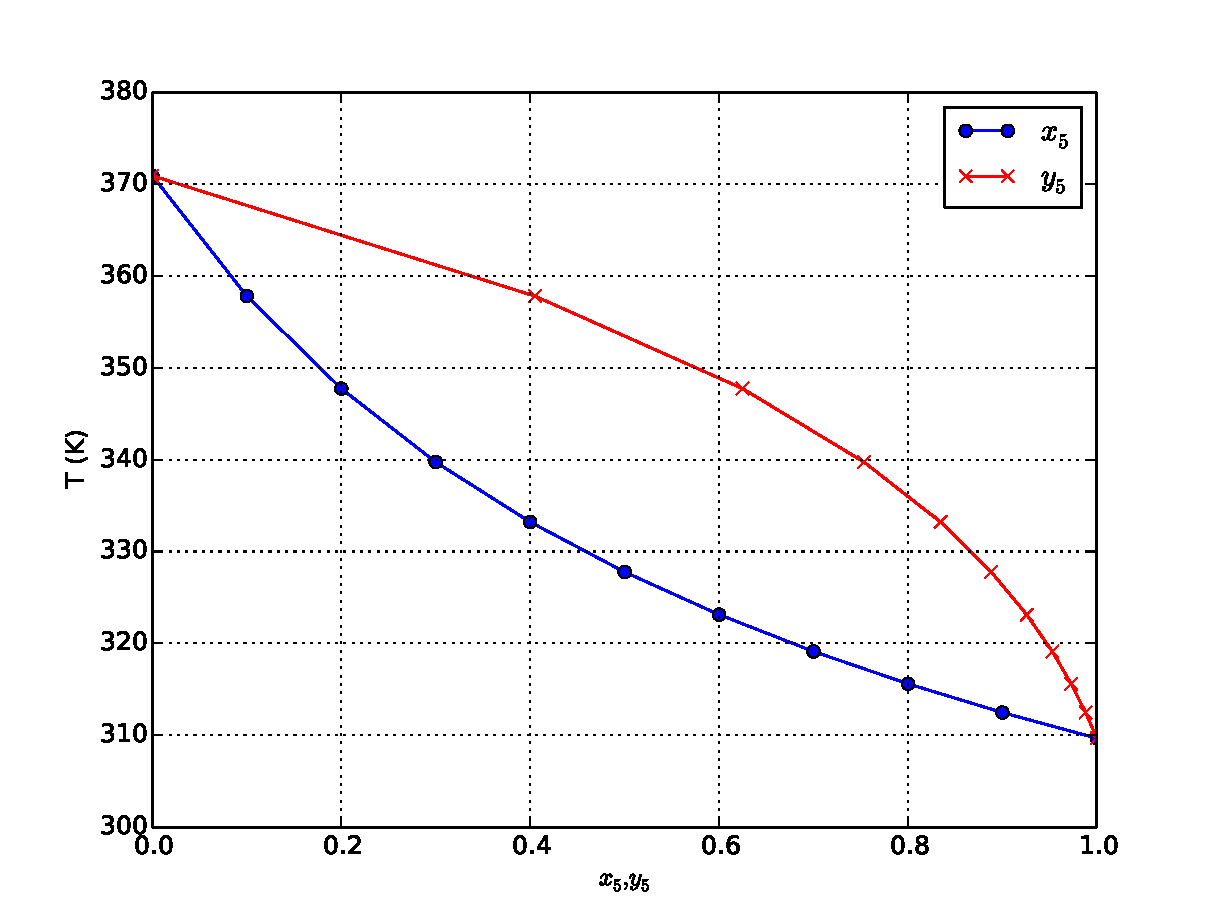
\includegraphics[width=.5\linewidth,clip]{./Figs/Mod4Ex2b}}}
         \caption{Example~\ref{Mod04Ex02}}
      \end{figure}
\clearpage
 % 
%%%
%%% EXAMPLE
%%%
   \item\label{Mod04Ex03} Estimate the bubble and dew point temperatures of a mixture of 25 mol-$\%$ of n-pentane, 45 mol-$\%$ of n-hexane and 30 mol-$\%$ of n-heptane at 1.013 bar. Given $P^{\text{sat}}$ relation,
    \begin{displaymath}
      \ln{P_{i}^{\text{sat}}} = A_{i} - \frc{B_{i}}{RT}
    \end{displaymath}
    with $A_{nC_{5}}=10.422$, $A_{nC_{6}}=10.456$, $A_{nC_{7}}=11.431$, $B_{nC_{5}}=26799 \text{ J.mol}^{-1}$, $B_{nC_{6}}=29676 \text{ J.mol}^{-1}$ and $B_{nC_{7}}=35200 \text{ J.mol}^{-1}$. Also [$P$] = bar and [$T$] = K.

% SOLUTION
 \noindent{\bf Solution:} Assuming the solution is ideal and the gas phase behaves as an ideal gas (\ie low/room pressure), Raoult's law can be used,
    \begin{displaymath}
       x_{i}P_{i}^{\text{sat}} = y_{i}P = P_{i} \;\;\text{ with }\;\; \summation[x_{i}P_{i}^{\text{sat}}]{i}{} = \summation[P_{i}]{i}{} = P, \;\summation[x_{i}]{i}{}=1=\summation[y_{i}]{i}{}.
    \end{displaymath}
    For the bubble point, the procedure is:
    \begin{enumerate}[i)]
       \item choose an initial guess for the bubble point temperature, $T^{\text{guess}}$;
       \item calculate $y_{i}=\frc{x_{i}P_{i}^{\text{sat}}}{P}$;
       \item then:
           \begin{itemize}
              \item if $\summation[y_{i}]{i}{} = 1 \;\;\Rightarrow \;\; T^{\text{guess}} = T$;
              \item if $\summation[y_{i}]{i}{} > 1 \;\;\Rightarrow \;\; T^{\text{guess}} > T \;\; \Rightarrow\;\; \text{adjust } T^{\text{guess}}$;
              \item if $\summation[y_{i}]{i}{} < 1 \;\;\Rightarrow \;\; T^{\text{guess}} < T \;\; \Rightarrow\;\; \text{adjust } T^{\text{guess}}$.
           \end{itemize}
    \end{enumerate}
    Thus, for this problem,
    \begin{displaymath}
        \summation[y_{i}]{i}{} = 1\;\; \Longleftrightarrow \;\; \frc{x_{5}P_{5}^{\text{sat}}}{P} + \frc{x_{6}P_{6}^{\text{sat}}}{P} + \frc{x_{7}P_{7}^{\text{sat}}}{P} = 1,
    \end{displaymath}
    where $P_{i}^{\text{sat}}$ is a function of $T$, 
    \begin{displaymath}
        \frc{x_{5}\exp{\left(A_{5}-\frc{B_{5}}{RT}\right)}}{P} + \frc{x_{6}\exp{\left(A_{6}-\frc{B_{6}}{RT}\right)}}{P} + \frc{x_{7}\exp{\left(A_{7}-\frc{B_{7}}{RT}\right)}}{P} = 1
    \end{displaymath}
    Using $T^{\text{guess}}=298.15$ K as initial guess, $T=334.9380$ K (bubble point temperature). Now, calculating the vapour composition, $y_{i}=\frc{x_{i}P_{i}^{\text{sat}}}{P}$ leads to,
    \begin{displaymath}
        y_{5} =0.5483,\;\; y_{6} = 0.3634\;\;\text{ and }\;\;y_{7} = 0.0883\;\;\Rightarrow\;\; \summation[y_{i}]{i}{} = 1.0000
    \end{displaymath}

\medskip
    For the dew point, the procedure is:
    \begin{enumerate}[i)]
       \item choose an initial guess for the dew point temperature, $T^{\text{guess}}$;
       \item calculate $x_{i}=\frc{y_{i}P}{P_{i}^{\text{sat}}}$;
       \item then:
           \begin{itemize}
              \item if $\summation[x_{i}]{i}{} = 1 \;\;\Rightarrow \;\; T^{\text{guess}} = T$;
              \item if $\summation[x_{i}]{i}{} > 1 \;\;\Rightarrow \;\; T^{\text{guess}} < T \;\; \Rightarrow\;\; \text{adjust } T^{\text{guess}}$;
              \item if $\summation[x_{i}]{i}{} < 1 \;\;\Rightarrow \;\; T^{\text{guess}} > T \;\; \Rightarrow\;\; \text{adjust } T^{\text{guess}}$.
           \end{itemize}
    \end{enumerate}
    Thus, for this problem,
    \begin{displaymath}
        \summation[x_{i}]{i}{} = 1\;\; \Longleftrightarrow \;\; \frc{y_{5}P}{P_{5}^{\text{sat}}} + \frc{y_{6}P}{P_{6}^{\text{sat}}} + \frc{y_{7}P}{P_{7}^{\text{sat}}} = 1,
    \end{displaymath}
    where $P_{i}^{\text{sat}}$ is a function of $T$, 
    \begin{displaymath}
        \frc{y_{5}P}{\exp{\left(A_{5}-\frc{B_{5}}{RT}\right)}} + \frc{x_{6}P}{\exp{\left(A_{6}-\frc{B_{6}}{RT}\right)}} + \frc{x_{7}P}{\exp{\left(A_{7}-\frc{B_{7}}{RT}\right)}}= 1
    \end{displaymath}
    Using $T^{\text{guess}}=298.15$ K as initial guess, $T=350.5857$ K (dew point temperature). Now, calculating the liquid composition, $y_{i}=\frc{x_{i}P_{i}^{\text{sat}}}{P}$ leads to,
    \begin{displaymath}
        x_{5} =0.0742\;\; x_{6} = 0.3463\;\;\text{ and }\;\;x_{7} = 0.5795\;\;\Rightarrow\;\; \summation[x_{i}]{i}{} = 1.0000
    \end{displaymath}


\clearpage
 % 
 % 
%%%
%%% EXAMPLE
%%%
   \item\label{Mod04Ex04} Estimate the bubble and dew point pressures of a mixture of 25 mol-$\%$ of n-pentane, 45 mol-$\%$ of n-hexane and 30 mol-$\%$ of n-heptane at 73$^{\circ}$C. Given $P^{\text{sat}}$ relation,
    \begin{displaymath}
      \ln{P_{i}^{\text{sat}}} = A_{i} - \frc{B_{i}}{RT}
    \end{displaymath}
    with $A_{nC_{5}}=10.422$, $A_{nC_{6}}=10.456$, $A_{nC_{7}}=11.431$, $B_{nC_{5}}=26799 \text{ J.mol}^{-1}$, $B_{nC_{6}}=29676 \text{ J.mol}^{-1}$ and $B_{nC_{7}}=35200 \text{ J.mol}^{-1}$. Also [$P$] = bar and [$T$] = K.

% SOLUTION
 \noindent{\bf Solution:}  For the bubble point, the mixture follows Raoult's law at 73$^{\circ}$C,
      \begin{displaymath}
          P = \summation[x_{i}P_{i}^{\text{sat}}]{i}{} = x_{5}P_{5}^{\text{sat}} + x_{6}P_{6}^{\text{sat}} + x_{7}P_{7}^{\text{sat}} = 1.413\text{ bar}
      \end{displaymath}
      This is the bubble point pressure at 346.15 K. The composition of the vapour phase is,
      \begin{displaymath}
             y_{i}=\frc{x_{i}P_{i}^{\text{sat}}}{P}
             \begin{cases}
                  y_{5} = 0.5370,\\
                  y_{6} = 0.3680,\\
                  y_{7} = 0.0950,
             \end{cases}
      \end{displaymath}
      leading to $\summation[y_{i}]{i}{} = 1.0000$.

\medskip

     For the dew point, the procedure is:
    \begin{enumerate}[i)]
       \item choose an initial guess for the dew point pressure, $P^{\text{guess}}$;
       \item calculate $x_{i}=\frc{Py_{i}}{P_{i}^{\text{sat}}}$;
       \item then:
           \begin{itemize}
              \item if $\summation[x_{i}]{i}{} = 1 \;\;\Rightarrow \;\; P^{\text{guess}} = P$;
              \item if $\summation[x_{i}]{i}{} > 1 \;\;\Rightarrow \;\; P^{\text{guess}} > P \;\; \Rightarrow\;\; \text{adjust } P^{\text{guess}}$;
              \item if $\summation[x_{i}]{i}{} < 1 \;\;\Rightarrow \;\; P^{\text{guess}} < P \;\; \Rightarrow\;\; \text{adjust } P^{\text{guess}}$.
           \end{itemize}
    \end{enumerate}
    Thus, for this problem,
    \begin{displaymath}
        \summation[x_{i}]{i}{} = 1\;\; \Longleftrightarrow \;\; \frc{y_{5}P}{P_{5}^{\text{sat}}} + \frc{y_{6}P}{P_{6}^{\text{sat}}} + \frc{y_{7}P}{P_{7}^{\text{sat}}} = 1,
    \end{displaymath}
    where $P_{i}^{\text{sat}}$ is a function of $T$ (which is known in this problem!).  Solving this equation leads to $P=0.8774$ bar (dew point pressure) with composition
    \begin{displaymath}
        x_{5} =0.0723\;\; x_{6} = 0.3418\;\;\text{ and }\;\;x_{7} = 0.5859\;\;\Rightarrow\;\; \summation[x_{i}]{i}{} = 1.0000
    \end{displaymath}


\clearpage
 % 
 % 
%%%
%%% EXAMPLE
%%%
   \item\label{Mod04Ex045} A liquid mixture of 25 mol-$\%$ n-pentane $\left(nC_{5}\right)$, 45 mol-$\%$ n-hexane $\left(nC_{6}\right)$ and 30 mol-$\%$ n-heptane $\left(nC_{7}\right)$ initially at 69$^{\circ}$C and a high pressure, is partially vaporised by isothermically lowering the pressure to  1.013 bar. Calculate the relative amounts of vapour and liquid in equilibrium and compositions.

% SOLUTION
 \noindent{\bf Solution:} This is a typical {\it flash} problem described by the figure,
    
  \begin{figure}[h]
     \begin{center}
         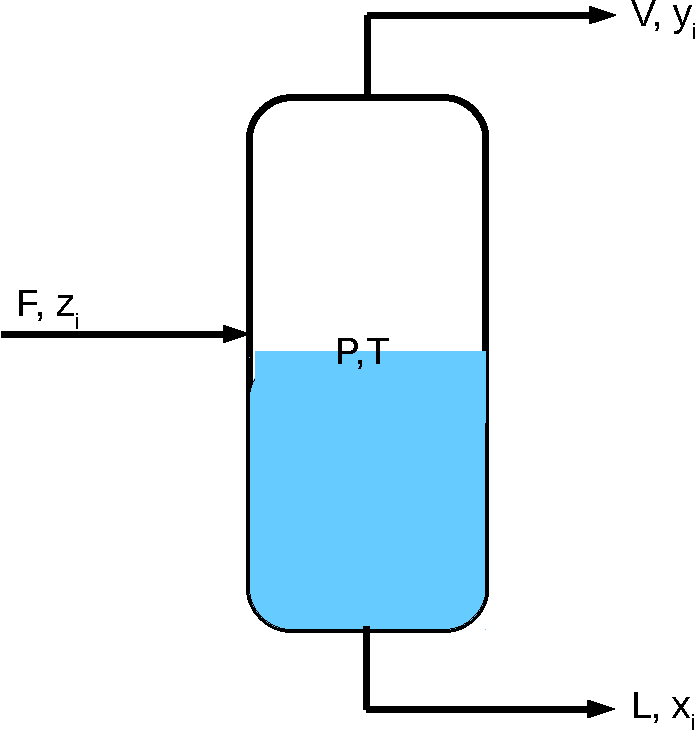
\includegraphics[width=.25\linewidth,clip]{./Figs/FlashDistillation}
     \end{center}
     \caption{Schematic of a flash distillation process, Example~\ref{Mod04Ex045}.}
  \end{figure}

From the given $P_{i}^{\text{sat}}$ relation at 69$^{\circ}$C,
   \begin{displaymath}
        \begin{cases}
            P_{5}^{\text{sat}} = 2.721 \text{ bar},\\ 
            P_{6}^{\text{sat}} = 1.024 \text{ bar},\\
            P_{7}^{\text{sat}} = 0.389 \text{ bar}.
        \end{cases}
   \end{displaymath}
Assuming ideal solution, $K_{i}$ for the three hydrocarbons can be readily obtained,
   \begin{displaymath}
        K_{i} = \frc{P_{i}^{\text{sat}}}{P} = \frc{y_{i}}{x_{i}},
          \begin{cases}
             K_{5} = 2.6861; \\
             K_{6} = 1.0109; \\
             K_{7} = 0.3840
          \end{cases}
   \end{displaymath}
   Therefore,
   \begin{displaymath}
       y_{5} = x_{5}K_{5},\;\;\;y_{6} = x_{6}K_{6},\;\;\;y_{7} = x_{7}K_{7},
   \end{displaymath}
    with the molar fraction constraints,
    \begin{displaymath}
        \begin{cases}
            x_{5}+x_{6}+x_{7} = 1,\\ 
            y_{5}+y_{6}+y_{7} = 1, \\
            F = V + L
        \end{cases}
   \end{displaymath}
   Assuming $F=1$, the mass balance of the individual components in equilibrium are
    \begin{displaymath}
        \begin{cases}
            x_{5}L + y_{5}V = z_{5} = 0.25 \\
            x_{6}L + y_{6}V = z_{6} = 0.45 \\
            x_{7}L + y_{7}V = z_{7} = 0.30            
        \end{cases}
   \end{displaymath}
   these relation can be rewritten as $\left(\text{based on }y_{5}+y_{6}+y_{7} = 1,\; y_{i}=K_{i}x_{i} \;\text{ and } V= 1-L\right)$
    \begin{displaymath}
        \begin{cases}
            x_{5}L + y_{5}V = z_{5} = 0.25 \;\Longrightarrow\; x_{5}\left[L\left(1-K_{5}\right)+K_{5}\right] = 0.25 \\
            x_{6}L + y_{6}V = z_{6} = 0.45 \;\Longrightarrow\; x_{6}\left[L\left(1-K_{6}\right)+K_{6}\right] = 0.45 \\
            x_{7}L + y_{7}V = z_{7} = 0.30 \;\Longrightarrow\; x_{7}\left[L\left(1-K_{7}\right)+K_{7}\right] = 0.30
        \end{cases}
   \end{displaymath}


   Now the molar fraction constraint of the liquid phase $x_{5}+x_{6}+x_{7} = 1$, is
   \begin{displaymath}
        \frc{0.25}{L\left(1-K_{5}\right)+K_{5}} + \frc{0.45}{L\left(1-K_{6}\right)+K_{6}} + \frc{0.30}{L\left(1-K_{7}\right)+K_{7}} = 1
   \end{displaymath}
   This expression has just one unknown, $L$, as a cubic polynomial. Solving with initial guess $L^{\text{guess}}=0.50$ leads to $L=0.5748$.  Now using 
    \begin{displaymath}
        \begin{cases}
            x_{5}L + y_{5}V = z_{5} = 0.25 \;\Longrightarrow\; x_{5}\left[L\left(1-K_{5}\right)+K_{5}\right] = 0.25  \;\Longrightarrow\;  x_{5} = 0.1456 \\
            x_{6}L + y_{6}V = z_{6} = 0.45 \;\Longrightarrow\; x_{6}\left[L\left(1-K_{6}\right)+K_{6}\right] = 0.45  \;\Longrightarrow\;  x_{6} = 0.4479 \\
            x_{7}L + y_{7}V = z_{7} = 0.30 \;\Longrightarrow\; x_{7}\left[L\left(1-K_{7}\right)+K_{7}\right] = 0.30  \;\Longrightarrow\;  x_{7} = 0.4065 
        \end{cases}
   \end{displaymath}
   leading to $\summation[x_{i}]{i}{} = 1.0000$. Molar fraction of the vapour phase is $V= 1-L=0.4252$, resulting in
    \begin{displaymath}
        \begin{cases}
            y_{5} = K_{5}x_{5} \;\Longrightarrow\; y_{5} = 0.3911 \\
            y_{6} = K_{6}x_{6} \;\Longrightarrow\; y_{6} = 0.4528 \\
            y_{7} = K_{7}x_{7} \;\Longrightarrow\; y_{7} = 0.1561 
        \end{cases}
   \end{displaymath}
    with $\summation[y_{i}]{i}{} = 1.0000$
 % 

%
\end{enumerate}
